\documentclass[a4paper, openright, 11pt, titlepage]{report}
\usepackage[table,xcdraw]{xcolor}
\usepackage[T1]{fontenc}
\usepackage[utf8]{inputenc}
\usepackage{lmodern}
\usepackage[spanish]{babel}
\usepackage{amssymb}
\usepackage{amsmath}
\usepackage{amsthm}
\usepackage[all]{xy}
\usepackage{graphicx}
\usepackage{enumerate}
\usepackage[none]{hyphenat}
\usepackage{caption}
\usepackage{mathptmx}
\setlength{\parskip}{0.5mm}
\usepackage{float}
\usepackage{appendix}
\usepackage{subfig}
\usepackage{wrapfig}
%\usepackage[usenames]{color}
%\usepackage{caption}
%\usepackage{subcaption}
\usepackage{hyperref}
\usepackage{multirow}
\usepackage{fancyhdr}


% \addbibresource{lib/lilylib/oll-lib/full.ily}
\usepackage{lilyglyphs}

\usepackage[minimal]{leadsheets}
\useleadsheetslibraries{musicsymbols}
\usepackage{musicography}
% \musWhole es la redonda
% \musHalf es la blanca
% \musQuarter es la negra
% \musEighth es la corchea
% \musSixteenth semicorchea

\usepackage{abc}
\usepackage{musixtex}

% \usepackage{wasysym}
% \usepackage{harmony}
% \usepackage{musixtex}

\usepackage[usenames]{color}
\usepackage[table]{xcolor}

\definecolor{acento}{rgb}{0.74, 0.83, 0.9}
    
% Para definir colores:

\definecolor{contexto}{RGB}{193,0,0}
\definecolor{actividades}{RGB}{0,124,0}
\definecolor{profesor}{RGB}{200,0,100}
\definecolor{personal}{RGB}{0,0,250}
\definecolor{participantes}{RGB}{200,100,0}
\definecolor{otros}{RGB}{300,200,0}

\usepackage[left=3cm,top=2.5cm,right=3cm,bottom=2.5cm,bindingoffset=0.5cm]{geometry}

\pretolerance=2000
\tolerance=3000

%================================================================
%Poner el título del teorema en negrita:
\makeatletter
\def\th@plain{%
  \thm@notefont{}% same as heading font
  \itshape % body font
}
\def\th@definition{%
  \thm@notefont{}% same as heading font
  \normalfont % body font
}
\makeatother
%================================================================

\newtheorem{propo}{Proposition}[section]
\newtheorem{teor}[propo]{Teorema}
\newtheorem{conje}[propo]{Conjeture}
\newtheorem{lema}[propo]{Lemma}
\newtheorem{corol}[propo]{Corolary}
\theoremstyle{definition}\newtheorem{defin}[propo]{Definition}
\theoremstyle{definition}\newtheorem{obser}[propo]{Remark}
\theoremstyle{definition}\newtheorem{ejem}[propo]{Ejemplo}
\theoremstyle{definition}\newtheorem{algoritmo}[propo]{Algoritmo}

\renewcommand{\thesubsubsection}{\thesubsection.\alph{subsubsection}}

\newcommand{\K}{\mathbb{K}}
\newcommand{\Pn}{\mathbb{P}}
\newcommand{\U}{\mathcal{U}}
\DeclareMathOperator{\Sing}{Sing} 
\DeclareMathOperator{\Sm}{Sm}
\DeclareMathOperator{\rk}{rank} 
\DeclareMathOperator{\mult}{mult} 
\DeclareMathOperator{\Card}{Card} 
\DeclareMathOperator{\Pic}{Pic} 

\renewcommand{\baselinestretch}{1.5}
\usepackage{vmargin}

\setpapersize{A4}
% \setmargins{2.5cm}       % margen izquierdo
% {1.5cm}                        % margen superior
% {16.5cm}                      % anchura del texto
% {23.42cm}                    % altura del texto
% {10pt}                           % altura de los encabezados
% {1cm}                           % espacio entre el texto y los encabezados
% {0pt}                             % altura del pie de página
% {2cm}


\title{Tarea Procesos y Contextos Educativos.}
\author{Elena Alcaide Pérez}
\begin{document}
\sloppy

% \begin{titlepage}

% \begin{center}
% % \vspace*{-1in}
% % \begin{figure}[htb]
% % \begin{center}
% % 
\includegraphics[width=5cm]{escudo}
% % \end{center}
% % \end{figure}


% % \begin{figure}[htb]
% %  \centering
% %  
\includegraphics[width=8cm]{./escudo}
% %  % escudo.png: 1476x1692 pixel, 100dpi, 37.49x42.98 cm, bb=0 0 1063 1218
% % \end{figure}


% UNIVERSIDAD NACIONAL DE EDUCACIÓN A DISTANCIA\\
% \vspace*{0.15in}
% FACULTAD DE EDUCACIÓN\\
% \vspace*{0.2in}
% Máster Universitario en Formación del Profesorado 
% de Educación Secundaria Obligatoria y Bachillerato, Formación Profesional y Enseñanza de Idiomas.\\
% \textsc{Especialidad en Matemáticas.}\\
% \vspace*{0.4cm}
% \large{\textsc{Tutora: ESTIBALITZ DURAND CARTAGENA}}\\

% \vspace*{0.3in}

% \begin{figure}[H]
%  \centering
%  
\includegraphics[width=8cm]{Images/escudo.png}
% %  escudo.png: 1476x1692 pixel, 100dpi, 37.49x42.98 cm, bb=0 0 1063 1218
% \end{figure}
% % \vspace*{0.6in}
% \vspace*{0.2in}
% \begin{LARGE}
% \textbf{Las Matemáticas de la Música: un proyecto interdisciplinar.}\\
% \end{LARGE}
% \vspace*{0.3in}
% \rule{80mm}{0.1mm}\\
% \vspace*{0.1in}
% \begin{LARGE}
% Elena Alcaide Pérez\\
% \end{LARGE}
% \vspace*{0.2in}
% \rule{80mm}{0.1mm}\\
% \vspace*{0.1in}
% \end{center}
% \end{titlepage}
\begin{titlepage}

\begin{center}
UNIVERSIDAD NACIONAL DE EDUCACIÓN A DISTANCIA\\
\vspace*{0.15in}
FACULTAD DE EDUCACIÓN\\
\vspace*{0.2in}
Máster Universitario en Formación del Profesorado 
de Educación Secundaria Obligatoria y Bachillerato, Formación Profesional y Enseñanza de Idiomas.\\
\textsc{Especialidad en Matemáticas.}\\
\vspace*{0.4cm}
\begin{LARGE}
\textbf{Las Matemáticas de la Música: un proyecto interdisciplinar.}\\
\end{LARGE}
\vspace*{0.3in}
\rule{80mm}{0.1mm}\\
\vspace*{0.1in}
\begin{LARGE}
Elena Alcaide Pérez\\
\end{LARGE}
\vspace*{0.2in}
\rule{80mm}{0.1mm}\\
\begin{figure}[H]
 \centering
 
\includegraphics[width=7cm]{Images/escudo.png}
\end{figure}
% \vspace*{0.6in}
\vspace*{0.2in}
\vspace*{0.1in}


\large{\textsc{Tutora: ESTIBALITZ DURAND CARTAGENA}}\\

\vspace*{0.3in}
\end{center}
\end{titlepage}
\newpage
\pagenumbering{Roman}
$\ $
\thispagestyle{empty} % para que no se numere esta pagina

\section*{Resumen} % si no queremos que añada la palabra "Capitulo"
\addcontentsline{toc}{section}{Resumen} % si queremos que aparezca en el índice
\markboth{RESUMEN}{RESUMEN} % encabezado
En el presente Trabajo de Fin de Máster se presentan algunos aspectos en los que se relacionan las Matemáticas y la Música. Además, se propone un proyecto interdisciplinar para llevar a cabo en un curso escolar con alumnos de 1º de Bachillerato basado en realizar actividades que relacionen estas dos disciplinas en cada uno de los bloques del currículo de este curso. Para ello, se han diseñado varias actividades describiendo, en cada una de ellas, los conceptos a enseñar, la metodología propuesta, la temporalización y los recursos necesarios.\\\\
Por otra parte, se ha pedido a dos profesionales relacionados con este campo su opinión acerca de la utilización de la Música en el aula y, en particular, sobre el uso de actividades interdisciplinares que relacionen las Matemáticas con otras asignaturas. El propósito de estas entrevistas es el de obtener  argumentos y criterios profesionales que justifiquen este proyecto 
interdisciplinar.
\section*{Abstract}
This Final Master Project presents some aspects in which the subjects of Mathematics and Music are related. Besides, an interdisciplinary project to be carried out during a school year with students of first course of “Bachillerato” is proposed. This project would be accomplished doing different activities that relate these two disciplines in each of the curricular blocks of this course. In order to do that, several tasks have been designed describing in each of them the concepts to be taught, the proposed methodology, the timing as well as the necessary resources.\\\\
On the other hand, two professionals related to this field have been asked for their opinion on the use of music in the classroom and, more specifically, on the use of interdisciplinary activities that connect mathematics with other subjects. The aim of these interviews is to obtain professional arguments and criteria to justify this interdisciplinary project.

\tableofcontents % indice de contenidos

\cleardoublepage
\addcontentsline{toc}{chapter}{Lista de figuras} % para que aparezca en el indice de contenidos
\listoffigures % indice de figuras

\cleardoublepage
\addcontentsline{toc}{chapter}{Lista de tablas} % para que aparezca en el indice de contenidos
\listoftables % indice de tablas
\newpage
\chapter{Introducción}
\pagenumbering{arabic}
\section{Introducción}
\pagestyle{fancy}
\fancyhf{}
\lhead[\textit{CAPÍTULO \thechapter}]{\textit{CAPÍTULO \thechapter}}
\rhead[\textit{\rightmark}]{\textit{\rightmark}}
\cfoot{\thepage}
La estrecha relación que existe entre las Matemáticas y la Música ha fascinado durante siglos tanto a músicos, que en ocasiones han incorporado procesos matemáticos en sus obras, como a matemáticos, algunos de los cuales estudiaban la Música a partir de sus conocimientos en esta ciencia.\\\\
Haciendo un análisis de la situación actual de estas dos disciplinas en la educación española, la autora ha observado que, por un lado, la Música es una asignatura que en la mayoría de institutos es considerada como secundaria, y por otra, las Matemáticas se convierten en una ciencia que los alumnos intentan aprender de memoria, sin darse cuenta de todas las aplicaciones que tiene en la vida real y cotidiana.\\\\
En ese contexto, este trabajo surge del interés por conocer las relaciones que existen entre estas dos disciplinas y ofrecer distintas actividades que puedan ser usadas en el aula y aportar, de esta forma, material que resulte útil al profesorado de Matemáticas.\\\\
El trabajo se ha dividido en siete capítulos, siendo el primero esta introducción. Los cuatro siguientes están dedicados a mostrar la relación entre la Música y las Matemáticas en distintos ámbitos: creación de escalas, sistemas de afinación, geometría y ritmos.\\
En el sexto capítulo y con el fin de convencer a los alumnos de la relación que existe entre estas dos disciplinas, se describen distintas actividades que pueden ser aplicadas durante el curso en diferentes bloques del currículo de 1º de Bachillerato, según el RD 1105/2014, de 26 de diciembre, por el que se establece el currículo básico de la Educación Secundaria Obligatoria y del Bachillerato. (BOE, \cite{boe}).\\\\
De esta forma, el profesor podrá enseñar conceptos básicos de Música a los alumnos e impartirá la asignatura de Matemáticas de una forma distinta, innovadora y original, demostrando a los estudiantes algo que no suelen tener en cuenta: las Matemáticas realmente están en todas partes.\\\\
El objetivo principal de este proyecto interdisciplinar es el de que los alumnos terminen el curso habiendo aprendido conceptos básicos musicales y habiendo comprendido la importancia que tienen las Matemáticas en un campo tan cercano a ellos.\\\\
Para finalizar, se presenta en el último capítulo las conclusiones que se han obtenido de este Trabajo de Fin de Máster, así como algunas líneas de trabajo futuras.
\section{Justificación}
Durante el periodo de prácticas, se ha podido observar que los alumnos aprenden las mecánicas de resolución de ejercicios de Matemáticas de memoria y que no entienden para qué puede servirles en el futuro.\\
En concreto y en una de las clases, los alumnos pidieron ayuda al profesor de Matemáticas con un ejercicio de física. El docente lo resolvió razonando de forma matemática (sin utilizar las fórmulas físicas) y los alumnos se quedaron asombrados de que estas dos ciencias realmente tuvieran tanta relación.\\
Esto fue, en gran medida, lo que consiguió motivar a la autora del trabajo a pensar actividades y diferentes metodologías didácticas que relacionaran las Matemáticas con las distintas disciplinas que estudian los alumnos durante el curso.\\
En particular, la elección de la Música fue puramente personal, por el propio amor que se tiene por este arte y, sobre todo, porque aunque actualmente no se considera una ciencia, en el pasado fue una rama de las Matemáticas. Convendría que los alumnos supieran que la Música que escuchan día a día tiene su fundamentación teórica en esa ciencia.\\\\
Por otra parte, estudios científicos desarrollan la tesis de que el saber tocar un instrumento y poder leer Música es de gran ayuda para la comprensión de las Matemáticas, pues, como describe Jauset Berrocal: ``\textit{el procesamiento de ambas materias lo realizan las mismas áreas cerebrales''}. (2008, J.A. Jauset Berrocal, \cite{berrocal})
 
\section{Objetivos}
\begin{enumerate}
    \item Investigar y presentar la historia sobre la relación entre las Matemáticas y la Música.
    \item Desarrollar algunos de los conceptos musicales que pueden ser explicados con Matemáticas. 
    \item Ofrecer actividades y recursos educativos para utilizar en un aula de Matemáticas de 1º de Bachillerato.
    \item Plantear un proyecto educativo interdisciplinar para alumnos de 1º de Bachillerato que pueda ser usado en un curso escolar.
\end{enumerate}
\newpage
\chapter{Música en la Antigua Grecia}
Ya en la antigua Grecia, la escuela pitagórica descubrió la estrecha relación existente entre las Matemáticas y la Música. Tal y como afirma Páez Gutiérrez (2009, \cite{paez}):\\\\
\textit{``la relación entre la Música y las Matemáticas se inició por culturas antiguas como la caldea, la egipcia, la babilónica y la china, pero fueron los pitagóricos los que unieron la Música y las Matemáticas''}\\\\
Fueron ellos los primeros en darse cuenta que existían sonidos agradables al oído y que, curiosamente, las longitudes de las cuerdas que los producían estaban en ciertas proporciones simples: 2/1, 3/2, 4/3, etc. De hecho, fue a raíz de estos descubrimientos por lo que los pitagóricos consideraron la Música una parte de las Matemáticas y así aparece en el \textit{``tratado sobre la Música''}, escrito por Boecio en el s.VI d.C.\\\\
Boecio desarrolló en este texto los principios del Pitagorismo y, en particular, aquellos dedicados a la Música. Sus escrituras sobre esta materia fueron la base de toda la teoría musical elaborada durante el Medioevo en el Occidente Cristiano \cite{tomasini} (Tomasini, M.C. (2007)). Consideraba la Música como una de las ciencias que permitía al hombre alcanzar la sabiduría. Dichas ciencias estaban recogidas en el \textit{quadrivium} (cuádruple vía hacia la sabiduría) y eran: Música, aritmética, geometría y astronomía; todas ellas disciplinas de las Matemáticas, y como tales, estudiaban las relaciones entre los números, proporciones y razones.\\\\
Para sus investigaciones, Pitágoras utilizó el monocordio, un instrumento constituido, como su nombre indica, por una sola cuerda. El experimento consistía en tensar una cuerda de longitud determinada (l) e ir estableciendo relaciones simples dividiendo la cuerda en partes. A estos intervalos resultantes de las proporciones simples (1/2, 2/3 y 3/4) se les llamaban ``consonancias perfectas'' y consistían en intervalos en los que intervenían únicamente los números que componen \textit{la Tetraktys}.\\\\
% cuyas razones subyacentes estaban formadas solamente por pequeños números 1, 2, 3 y 4 -la Tetraktys-“. (Abdounur, p.63, \cite{abd})\\\\
La relación más sencilla (1/2) se obtenía dividiendo la cuerda por la mitad, de esta forma se tenían dos sonidos que se corresponden con un intervalo de octava: si la cuerda suelta determinaba la nota Do, al aplicar esta relación simple se obtenía de nuevo un Do, pero más agudo.\\
De la misma forma, si la medida utilizada es 2/3, el intervalo que se obtiene es una quinta (Do-Sol) y, por último, si la relación aplicada es 3/4, entonces se obtiene un intervalo de cuarta (Do-Fa). Se tiene el siguiente diagrama:
\begin{figure}[H]
    \centering
    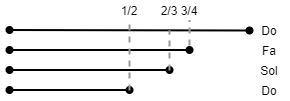
\includegraphics[scale = 0.7]{Images/Capítulo 2/diagrama1.png}
    \caption{Longitud de la cuerda que genera un sonido, su octava, su quinta y su cuarta.}
    %\label{fig:my_label}
\end{figure}
Estos intervalos, la octava, quinta y cuarta, fueron la base del sistema musical polifónico. Como ya se ha comentado, esto era debido a que los pitagóricos consideraban que solo estas proporciones estaban dentro del límite de la Tetraktys, o suma de los cuatro primeros números: $$1 + 2 + 3 + 4 = 10$$
A partir de estos descubrimientos, los pitagóricos construyeron la primera escala musical. Esto se explica en el siguiente apartado.
\chapter{Sistemas de afinación.}
\section{Sistema de afinación pitagórico.}
Una vez obtenidos los intervalos a partir de una única nota, los pitagóricos comenzaron a investigar qué ocurría si tomaban de referencia una de las notas recién descubiertas, es decir, comenzaron a establecer relaciones de proporcionalidad a partir de dichas notas. Con esta exploración, los pitagóricos descubrieron que la quinta de Sol era Re: al multiplicar el valor de Sol como quinta de Do $(\frac{3}{2})$ por él mismo, se obtiene $\frac{9}{4}$. Este valor es mayor que 2 y por tanto se sale de la octava en la que estaban operando pero, dado que al multiplicar por $\frac{1}{2}$ se obtiene la misma nota pero en otra octava, dividieron el resultado entre dos, obteniendo: $$\frac{3}{2}*\frac{3}{2} = \frac{9}{4} \Longrightarrow \frac{9}{4}*\frac{1}{2} = \frac{9}{8}$$
que, como se ha dicho, es la nota Re, quinta de Sol. \\
Si se continúa con este proceso se obtiene:
\begin{table}[H]
\centering
\begin{tabular}{c|c|c}
\hline
     Nota inicial & Operación & Nota resultante \\
     \hline \hline
     Sol & $\frac{3}{2}*\frac{3}{2} = \frac{9}{4} \Longrightarrow \frac{9}{4}*\frac{1}{2} = \frac{9}{8}$ & Re \\
     Re & $\frac{9}{4}*\frac{3}{2} = \frac{27}{8} \Longrightarrow \frac{27}{8}*\frac{1}{2} = \frac{27}{16}$ & La \\
     La & $\frac{27}{8}*\frac{3}{2} = \frac{81}{16} \Longrightarrow \frac{81}{16}*\frac{1}{2^{2}} = \frac{81}{64}$ & Mi\\
     Mi & $\frac{81}{32}*\frac{3}{2} = \frac{243}{64} \Longrightarrow \frac{243}{64}*\frac{1}{2} = \frac{243}{128}$ & Si \\
     \hline
\end{tabular}
\caption{Cálculo de quintas.}
\label{tablaquintas}
\end{table}
Y, escribiendo las notas con sus correspondientes proporcionalidades en un pentagrama se obtiene:
\begin{figure}[H]
    \centering
    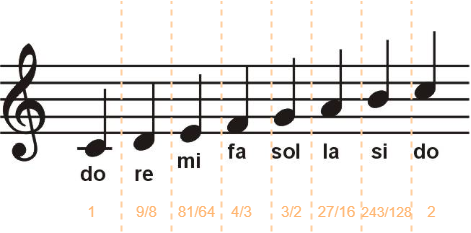
\includegraphics[width = 0.5\textwidth]{Images/Capítulo 3/pentagrama.png}
    \caption{Valor de cada nota musical respecto del primer Do .}
    %\label{fig:my_label}
\end{figure}
Si se dibuja la escala en el plano donde las $x$ son las notas de la escala y las $y$ son las proporciones calculadas para cada nota, se tiene el siguiente gráfico:
\begin{figure}[H]
    \centering
    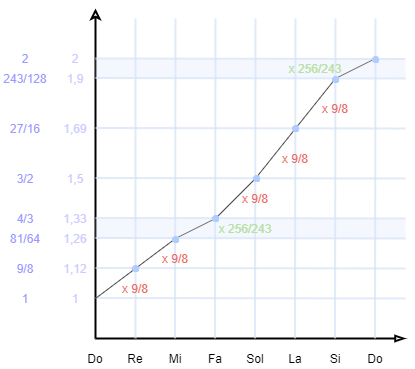
\includegraphics[width = 0.7\textwidth]{Images/Capítulo 3/graficoEscala1.png}
    \caption{Gráfico de la escala según proporciones de quintas.}
    %\label{fig:my_label}
\end{figure}
Si fuera un método de cálculo simétrico y cada nota estuviera a la misma distancia de la siguiente, se obtendría una recta parecida a $y = x$ pero está claro que no es un método perfecto:\\\\
Existen en realidad dos intervalos más pequeños que los demás: entre el Mi y el Fa y entre el Si y el Do, lo cual, si se observan las teclas de un piano, no es una coincidencia:
\begin{figure}[H]
    \centering
    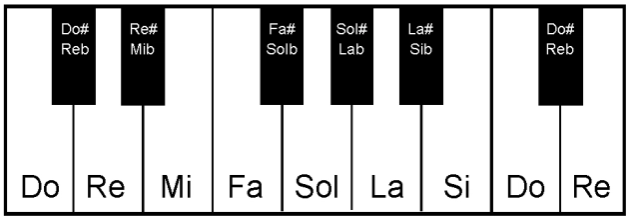
\includegraphics[scale = 0.5]{Images/Capítulo 3/teclasPiano.png}
    \caption{Teclas del piano.}
    %\label{fig:my_label}
\end{figure}
Los intervalos más pequeños corresponden a las teclas blancas del piano que no tienen tecla negra entre ellas: son los dos únicos intervalos de semitono que se encuentran en la escala natural. Y aquí se tiene el primer error de cálculo en este método de afinación: la distancia de semitono no es la mitad exacta de un tono: $$\frac{256}{243} = 1,053 \not= \sqrt{\frac{9}{8}} \simeq 1,06$$
En la gráfica también se puede observar que la diferencia entre las proporciones va aumentando en cada quinta (sin tener en cuenta los semitonos ya mencionados). De hecho, si se sigue el proceso añadiendo quintas, se obtienen sonidos intermedios (las teclas negras del piano) pero estas proporciones comienzan a ser menos homogéneas.\\
Aún así, si se continúa hasta completar 12 quintas se obtienen los 5 sonidos restantes que faltan para volver a llegar al sonido original cerrando así el conocido círculo de quintas:
\begin{figure}[H]
    \centering
    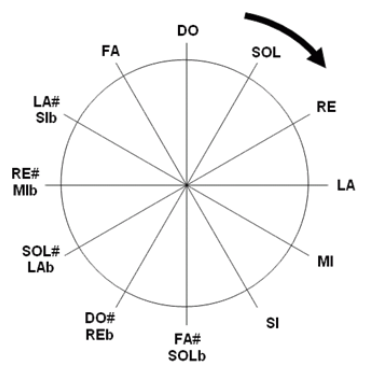
\includegraphics[scale = 0.7]{Images/Capítulo 3/quintas.png}
    \caption{Círculo de quintas.}
    %\label{fig:my_label}
\end{figure}
Sin embargo, la proporción que se obtiene realizando el mismo proceso que en el Cuadro \ref{tablaquintas} corresponde con un Do pero 7 octavas más arriba, es decir, se obtiene una proporción que, para que sea menor que 2, hay que multiplicarlo por $\frac{1}{2^{7}}$.\\
Sin embargo, no resulta \textbf{exactamente} el valor de Do original, de hecho difiere en centésimas, pero es obvio que si se multiplica $12$ veces por $\frac{3}{2}$ nunca se va a obtener una potencia de 2. Dicho de otra forma, 12 quintas no son 7 octavas: $$2^{7} = 128 \not= (\frac{3}{2})^{12} \simeq 129,746$$
Si se quiere cerrar el círculo completamente, una de las quintas debe medir un poco menos que el resto y por tanto no será perfectamente consonante. De hecho, se le denominaba \textit{quinta del lobo} por lo mal que sonaba. En el sistema que se ha explicado, se procuró situar esta quinta entre dos notas que no se manejasen habitualmente: Sol$\sharp$ y Mi$\flat$. 

Los anteriores errores descritos hicieron que se rechazara finalmente la afinación pitagórica y se investigaron distintos tipos hasta llegar al sistema temperado, el cual se utiliza actualmente.

\section{Sistema de afinación temperado.}
Antes de llegar a este sistema, a lo largo de la historia se han estudiado muchos otros, como por ejemplo: 
\begin{itemize}
    \item \textbf{Temperamento justo} o \textbf{temperamento mesotónico}. Fue el sistema de afinación más utilizado a partir del siglo XVI y estaba basado en la consonancia de 3ª. 
    \item \textbf{Temperamentos irregulares}. Se propusieron casi al mismo tiempo que el temperamento justo. Se llamaba así porque trataba de eliminar la quinta del lobo repartiendo esa proporción entre las otras quintas. Sin embargo, esta repartición se hacía de forma \textit{irregular}.
    \item \textbf{Sistema de Holder}, que dividía la distancia entre notas en unidades interválicas más pequeñas que el semitono.
\end{itemize}
Finalmente se propuso el \textbf{sistema temperado}, o temperamento igual, basado en 12 semitonos iguales y tiene en cuenta únicamente la consonancia de la 8ª, no como el pitagórico que consideraba tanto la 8º como la 5º.\\\\
Para comprender este sistema, lo primero que hay que comprobar es cuánto mide el intervalo de semitono:\\
Dependerá, en primer lugar de la frecuencia desde la que se parta y, dado que un intervalo es una proporción de frecuencias, se obtendrá el valor de la frecuencia de cada nota al multiplicar la nota anterior por dicha proporción. Por ejemplo, sea f la frecuencia de Do y p la proporción entre semitonos. La frecuencia de Do# se obtendrá como $f*p$. Para obtener la frecuencia de Re: $f*p^{2}$, y así sucesivamente.\\
Por tanto, se necesita completar una 8ª con 12 intervalos iguales y además que la proporción del semitono $(p)$, al multiplicarlo 12 veces consecutivas por una frecuencia base $(f)$, dé como resultado $2f$: el mismo sonido una octava más arriba. Es decir: $$f*p^{12} = 2f \longrightarrow p^{12} = 2 \longrightarrow p = \sqrt[12]{2} = 1,059$$

A continuación se muestran dos figuras: en la tabla \ref{calculos} aparece el cálculo de la proporción entre notas según el sistema pitagórico y el temperado, pudiendo comprobar así las diferencias de cálculo que existen entre ellos. En la segunda figura se puede apreciar esto gráficamente:
\begin{table}[H]
    \centering
    \begin{tabular}{|c|c|c|c|c|}
    \hline
         Nota & Semitono & Intervalo & Afinación pitagórica & Afinación temperada\\
         \hline
         \hline
         Do & 0 & Unísono & 1 & 1\\
         Do \# & 1 & Semitono & $\frac{2187}{2048} = 1,06787$ & $\sqrt[12]{2} = 1,05946$\\
         Re & 2 & 2ª Mayor & $\frac{9}{8} = 1,125$ & $\sqrt[12]{2^{2}} = 1,12246$\\
         Mi \textit{b} & 3 & 3ª menor & $\frac{32}{27} = 1,185185$ & $\sqrt[12]{2^{3}} = 1,18921$\\
         Mi & 4 & 3ª Mayor & $\frac{81}{64} = 1,26562$ & $\sqrt[12]{2^{4}} = 1,25992$\\
         Fa & 5 & 4ª justa & $\frac{4}{3} = 1,33333$ & $\sqrt[12]{2^{5}} = 1,33484$\\
         Fa \# & 6 & 4º Aumentada & $\frac{729}{512} = 1,51923$ & $\sqrt[12]{2^{6}} = 1,41421$\\
         Sol & 7 & 5ª Justa & $\frac{3}{2} = 1,5$ & $\sqrt[12]{2^{7}} = 1,49831$\\
         Sol \# & 8 & 5ª Aumentada & $\frac{6561}{4096} = 1,60181$ & $\sqrt[12]{2^{8}} = 1,58740$\\
         La & 9 & 6ª Mayor & $\frac{27}{16} = 1,6875$ & $\sqrt[12]{2^{9}} = 1,68179$\\
         Si \textit{b} & 10 & 7ª menor & $\frac{16}{9} = 1,77777$ & $\sqrt[12]{2^{10}} = 1,78179$\\
         Si & 11 & 7ª Mayor & $\frac{243}{128} = 1,89844$ & $\sqrt[12]{2^{11}} = 1,88775$\\
         Do & 12 & 8ª Justa & 2 & 2\\
         \hline
    \end{tabular}
    \caption{valores de las notas según afinación pitagórica y afinación temperada, siendo la nota base Do.}
    \label{calculos}
\end{table}
\begin{figure}[H]
    \centering
    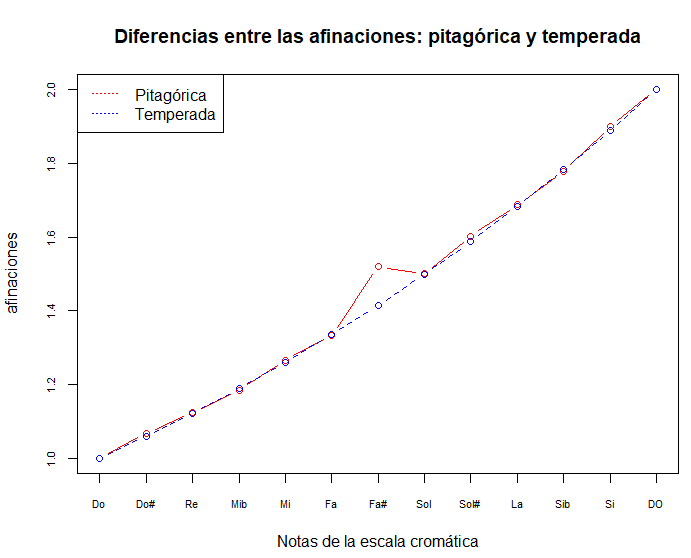
\includegraphics[scale = 0.8]{Images/Capítulo 3/graficoCromatica.png}
    \caption{Diferencias entre la afinación pitagórica y la temperada.}
    \label{grafica}
\end{figure}
En la Figura \ref{grafica}, tal y como se ha dicho, se pueden observar las diferencias de las notas de la escala cromática. Ya se ve en la tabla que las diferencias en los resultados de los cálculos difieren, en casi todos los casos, en centésimas. Sin embargo, en el caso de la nota Fa$\sharp$ difiere en una décima, lo cual aparece dibujado en el gráfico. Esto es debido a la quinta del lobo explicada anteriormente. \\\\
Ahora bien, se ha mencionado que el valor de la nota en este sistema de afinación viene definido por la frecuencia. A lo largo de la historia se han utilizado distintas medidas para hallar dichas frecuencias y, de hecho, cada compositor utilizaba para sus obras las frecuencias que le convenían, teniendo que afinar de nuevo los instrumentos cada vez que estas medidas cambiaban. Sin embargo, en 1939, en la Segunda conferencia Internacional para el Diapasón, se determinó (a nivel internacional) que la frecuencia de la nota La era 440 Hz.\\
De aquí y aplicando la fórmula descrita, se obtienen las frecuencias de cada nota que actualmente se utilizan:
\begin{table}[H]
    \centering
    \begin{tabular}{|c|c|}
    \hline
    Nota & Frecuencia\\
    \hline \hline
       Do & $261.6$\\
       Do \# & $277.18$\\
       Re & $293.66$\\
       Mi \textit{b} & $311.13$\\
       Mi & $329.63$\\
       Fa & $349.23$\\
       Fa \# & $369.99$\\
       Sol & $392.00$\\
       Sol \# & $415.30$\\
       La & $440.00$\\
       Si \textit{b} & $466.16$\\
       Si & $493.88$\\
       DO & $523.2$\\
       \hline
    \end{tabular}
    \caption{Frecuencias de las notas en Herzios.}
    %\label{tab:my_label}
\end{table}

\chapter{Geometría en la Música}
\section{Creación de escalas simétricas}
Uno de los conceptos más bonitos que relaciona la geometría y la Música es la creación de escalas bien formadas (del inglés: \textit{Well-Formed scales}) o escalas simétricas. A continuación, se dan ejemplos para después definir el concepto.\\\\
Si se toma la secuencia de quintas de la escala diatónica (Do-Sol-Re-La-Mi-Si-Fa) y se representa alrededor de una circunferencia de forma regular se tiene: 
\begin{figure}[H]
    \centering
    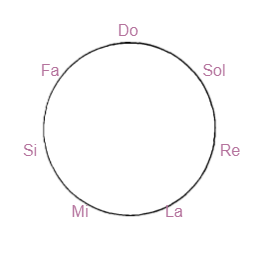
\includegraphics[scale = 0.7]{Images/Capítulo 4/circuloQuintas.png}
    \caption{Círculo de quintas con las 7 primeras notas.}
    %\label{fig:my_label}
\end{figure}
Estas notas se pueden unir de dos formas distintas:
\begin{figure}[H]
    \centering
    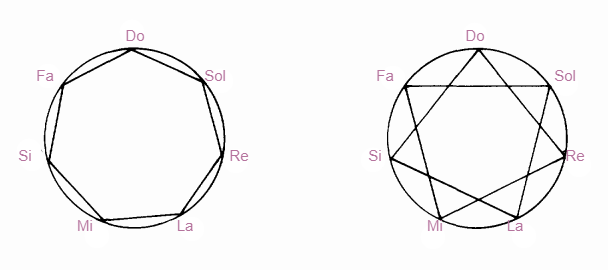
\includegraphics[scale = 0.7]{Images/Capítulo 4/diatonicaSimetrica.png}
    %\caption{Diferencias de la afinación pitagórica y la temperada.}
    %\label{fig:my_label}
\end{figure}
En la primera figura, cada nota ha sido conectada con su respectiva quinta y, en la segunda, cada nota con su consiguiente según el orden natural de la escala (Do-Re, Re-Mi, Mi-Fa,...).\\\\
El heptágono regular (figura de la izquierda) se ha construido comenzando por el Do, pero si se comenzara por cualquier otra nota, la figura seguiría siendo un heptágono. Dicho de otra forma, la figura que forman las notas de la escala diatónica unidas por quintas tiene siete grados de simetría rotacional. Además, es importante recordar que las notas guardan una relación de simetría entre ellas y se conectan consecutivamente por intervalos de quintas iguales.\\
La figura que surge al conectar las notas de la escala según su orden natural también tiene siete grados de simetría rotacional.\\
Cuando esto ocurre en ambas figuras se dice que la escala preserva la simetría del círculo de quintas.\\\\
Pero no se tiene por qué elegir las 7 primeras notas, se puede dibujar para cualquier número de intervalos de quintas, pero no siempre cumple esta cualidad. Por ejemplo, en el caso de elegir las 6 primeras quintas (Do-Sol-Re-La-Mi-Si):
\begin{figure}[H]
    \centering
    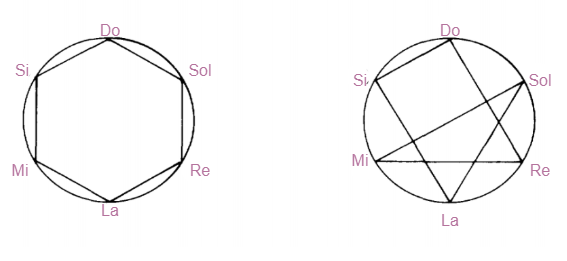
\includegraphics[scale = 0.7]{Images/Capítulo 4/seisQuintas.png}
    %\caption{Diferencias de la afinación pitagórica y la temperada.}
    %\label{fig:my_label}
\end{figure}
La primera figura, obviamente, es un hexágono regular y por tanto tiene seis grados de simetría rotacional, sin embargo la segunda figura no cumple esta propiedad.\\\\
Si se toman las 5 primeras quintas vuelve a cumplirse la propiedad, apareciendo la \textit{escala pentatónica}:
\begin{figure}[H]
    \centering
    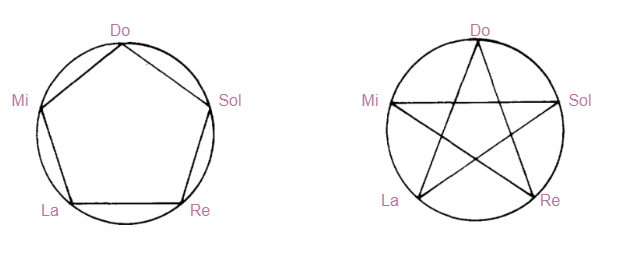
\includegraphics[scale = 0.7]{Images/Capítulo 4/cincoQuintas.png}
    %\caption{Diferencias de la afinación pitagórica y la temperada.}
    %\label{fig:my_label}
\end{figure}
Esta condición de simetría hace que se puedan distinguir fácilmente dos tipos de escalas y, como consecuencia, se establece la siguiente definición:\\
Las escalas generadas por quintas consecutivas que preservan la simetría de la figura geométrica formada por la unión de las notas en su orden natural se denominan \textit{escalas bien formadas}.\\\\
Se ha explicado el concepto en base a las 7 primeras notas del círculo de quintas, sin embargo, si se toman todas las notas con sus respectivas alteraciones, también se obtienen \textit{escalas bien formadas}. La más famosa es la escala cromática: 
\begin{figure}[H]
    \centering
    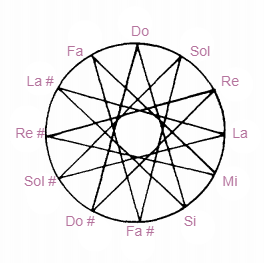
\includegraphics[scale = 0.7]{Images/Capítulo 4/circuloCromatica.png}
    %\caption{Diferencias de la afinación pitagórica y la temperada.}
    %\label{fig:my_label}
\end{figure}
La teoría de las \textit{escalas bien formadas} es una rama de las Matemáticas que apareció en la década de los 80, sin embargo, no es casualidad que a lo largo de la historia distintas culturas hayan utilizado estas escalas. La diatónica y cromática son base del sistema musical actual occidental. Los cantos gregorianos tempranos contenían melodías pentatónicas y se pueden encontrar estas escalas (pentatónica) en la Música tradicional nativa americana, africana y del sur de Asia.\\
Si se siguen añadiendo notas al círculo, las siguientes estrellas regulares que aparecen son las que involucran 17 y 53 notas que son, respectivamente, las que se usaban en las civilizaciones árabe y china de la antigüedad.
\section{Geometría y composición}
Hasta ahora se han explicado algunos conceptos de la teoría musical a partir de las Matemáticas. En este apartado se van a dar ejemplos de compositores que han utilizado las Matemáticas en sus obras, en concreto las transformaciones en el plano.\\ Se sabe bien que este tipo de movimientos aparece constantemente en el arte de la pintura. Los artistas las han utilizado a lo largo de la historia, por ejemplo \textit{El hombre de Vitruvio} de Leonardo da Vinci, es simétrico respecto de un eje central:
\begin{figure}[H]
    \centering
    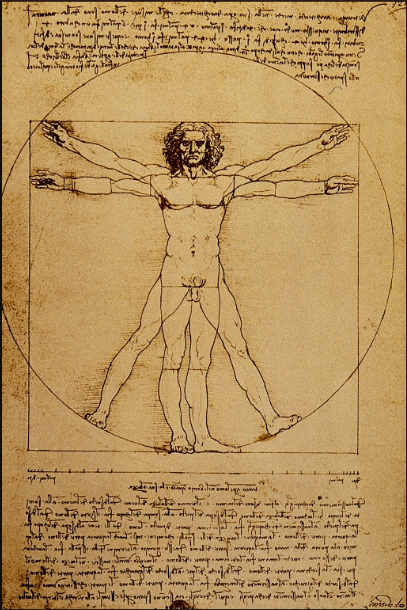
\includegraphics[width = 0.4\textwidth]{Images/Capítulo 4/davinci.png}
    \caption{\textit{Hombre de Vitruvio}. Imagen de \cite{vitruvio}}
\end{figure}
O por ejemplo y teniendo en cuenta que el tema que se está tratando está relacionado con la Música, el mismo Johann Sebastian Bach diseñó su propio sello simétrico respecto de un eje vertical: 
\begin{figure}[H]
    \centering
    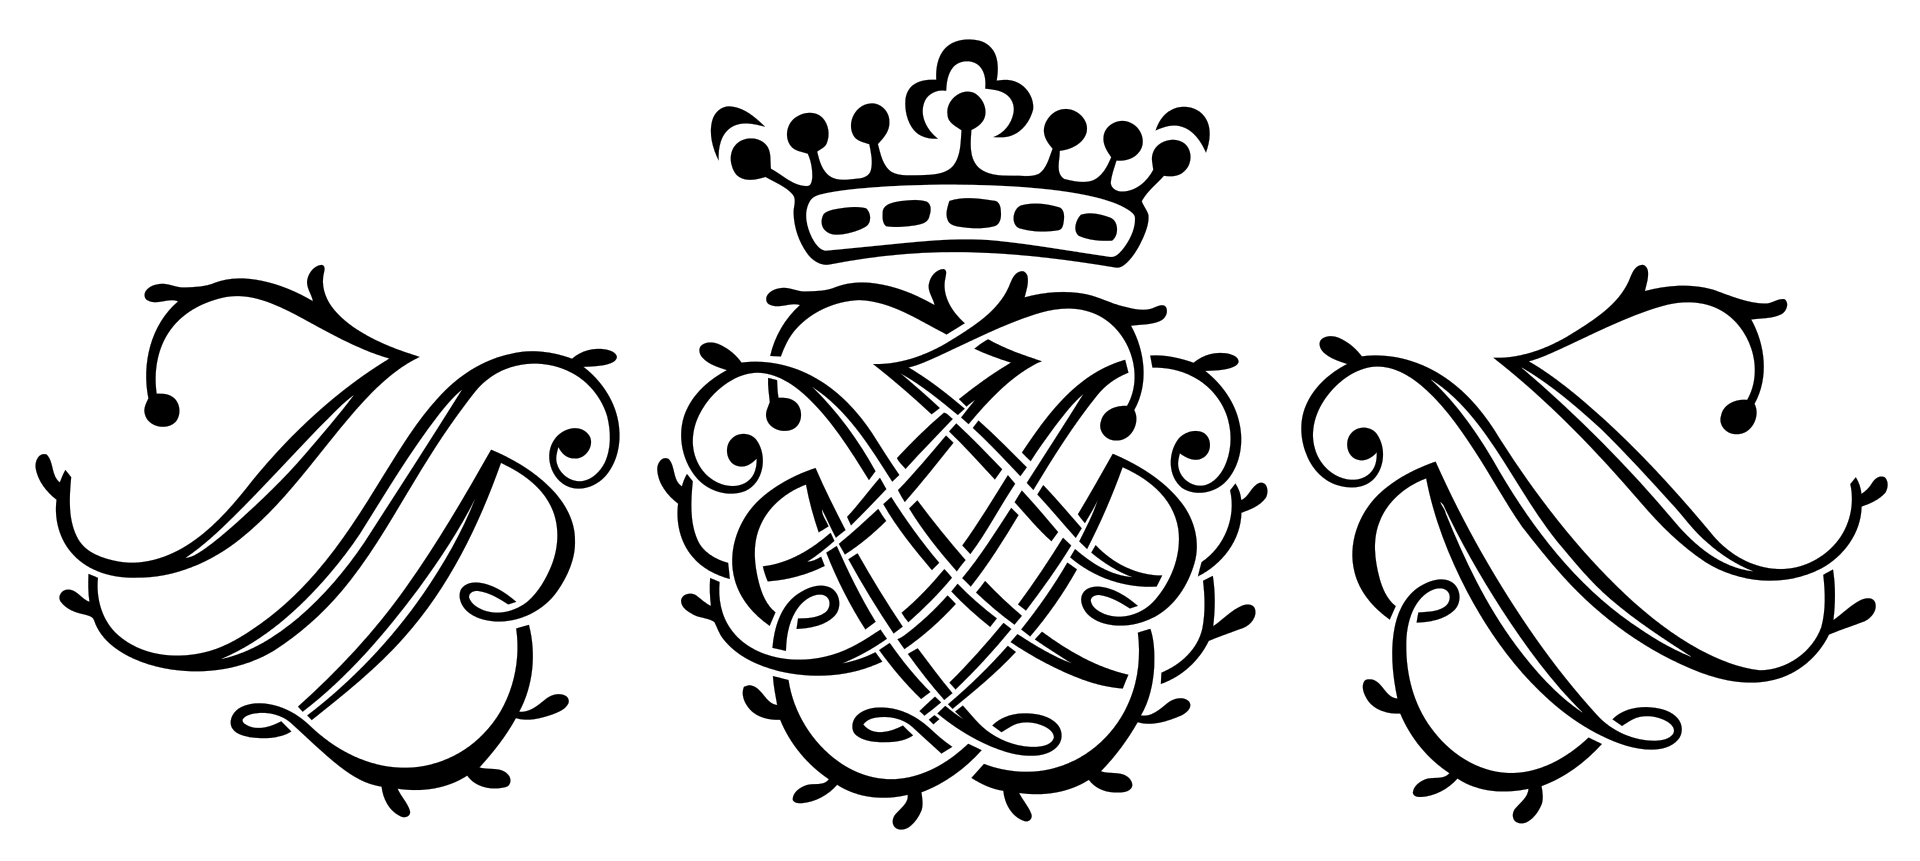
\includegraphics[width = 0.5\textwidth]{Images/Capítulo 4/selloBach.png}
    \caption{Sello de Johann Sebastian Bach. \cite{sello}}
\end{figure}
También en los mosaicos de la Alhambra de Granada aparecen estas transformaciones. Muchos de ellos se consiguen a partir de la rotación y traslación de distintas figuras geométricas:
\begin{figure}[H]
    \centering
    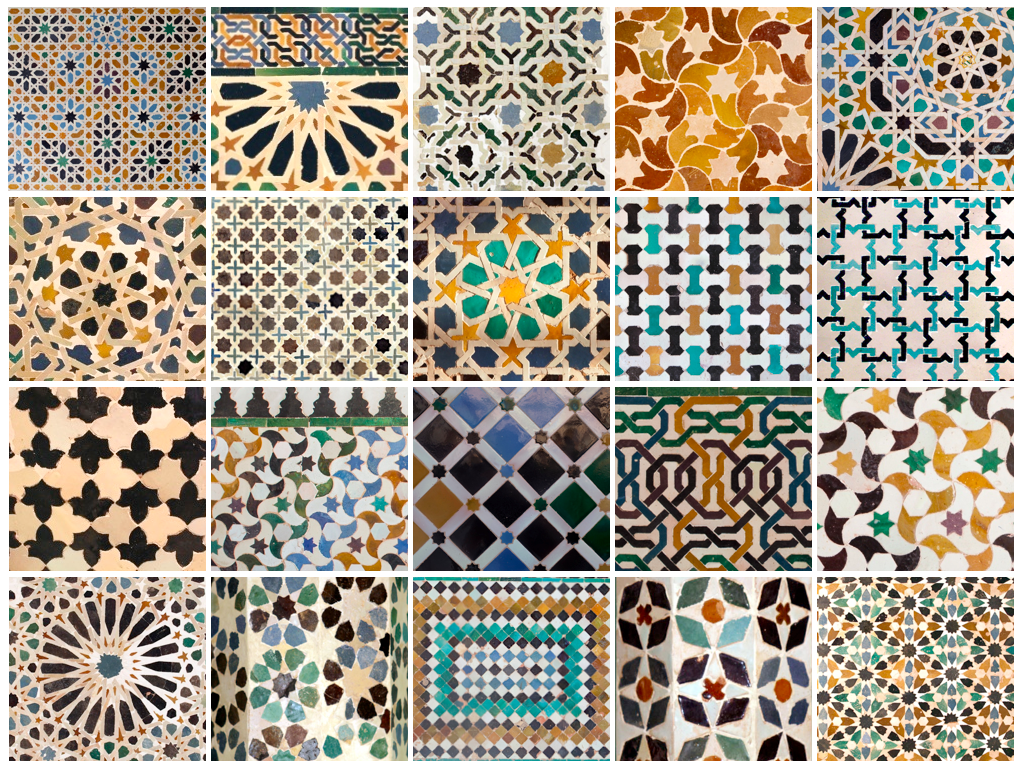
\includegraphics[width = 0.6\textwidth]{Images/Capítulo 4/alhambra.png}
    \caption{Mosaicos de la Alhambra de Granada. Imagen de \cite{alhambra}}
\end{figure}
Sin embargo, y aunque la utilización de las Matemáticas no es tan conocida en el arte de la Música, muchos compositores, algunos de ellos muy famosos, las han usado para crear sus obras.\\\\
Por otra parte, es importante tener muy claro tanto el concepto de \textit{transformación} como los diferentes tipos de transformación que se pueden considerar y que aparecen en determinadas obras musicales.\\\\
Se dice que una figura en el plano sufre una \textit{transformación} cuando, mediante operaciones Matemáticas, se puede obtener una nueva figura a partir de la dada. Para este trabajo interesan aquellas que no varían ni el tamaño ni la forma del objeto. Estas transformaciones se conocen como \textit{movimientos en el plano} o \textit{isometrías} y son:
\begin{itemize}
    \item \textbf{Traslación.} Se denomina \textit{traslación} T de vector $\Vec{v}$ a una transformación que asocia cada punto P del plano con otro punto P' tal que: $$P' = T(P) = P + \Vec{v}$$
    Las traslaciones son movimientos del plano ya que conservan su forma y tamaño y, además, son directos ya que conservan también la orientación.
    \begin{figure}[H]
        \centering
        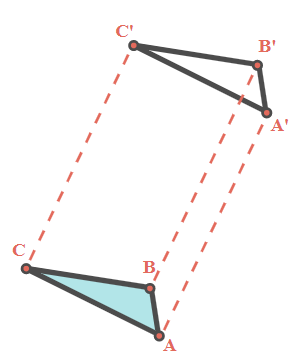
\includegraphics[width = 0.25\textwidth]{Images/Capítulo 4/traslacion.png}
        \caption{Traslación de un objeto. Imagen de \cite{sangaku}}
    \end{figure}
    \item \textbf{Rotación.} Las rotaciones o giros son, al igual que las traslaciones, movimientos directos.\\
    Se define una \textit{rotación} en el plano de centro O y ángulo $\alpha$ al movimiento que hace corresponder a un punto P otro punto P' de forma que: 
    $$\Vec{PO} = \Vec{P'O} \hspace{0.3cm} \text{y} \hspace{0.3cm} \hat{POP'} = \alpha$$
        \begin{figure}[H]
            \centering
            \subfloat[Rotación de un punto en el plano.]{
                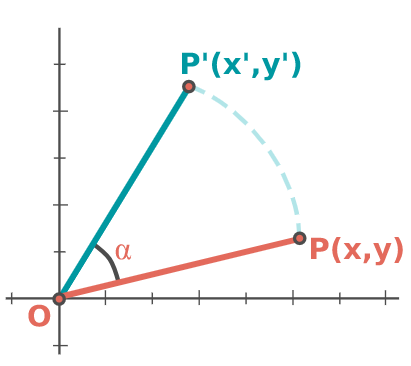
\includegraphics[width = 0.3\textwidth]{Images/Capítulo 4/rotacion.png}}
            \subfloat[Rotación de un objeto.]{
                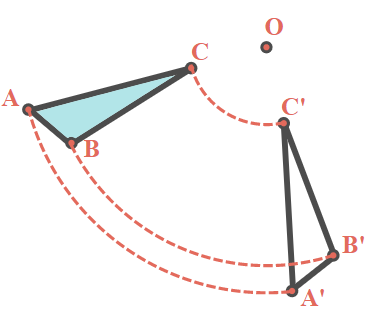
\includegraphics[width = 0.3\textwidth]{Images/Capítulo 4/rotacionObjeto.png}}
                \caption{Rotación de forma gráfica. Imagen de \cite{sangaku}}
        \end{figure}
    \item \textbf{Simetría axial} o simetría de reflexión. Se da cuando los puntos de una figura son simétricos respecto de un eje a los puntos de otra figura. Es decir, dado una recta $e$ llamada eje, a todo punto $P$ del plano le corresponde otro punto $P'$ tal que el eje es la mediatriz del segmento $\Vec{PP'}$.\\
    Este tipo de transformación es la que ocurre, por ejemplo, en un espejo. Se define como una \textit{isometría inversa} pues los objetos conservan las distancias entre los puntos y la forma pero la orientación es inversa. En la siguiente figura se puede observar la simetría de un punto respecto del eje X (a), respecto del eje Y (b) y la simetría de un objeto respecto de un eje cualquiera (c).
    \begin{figure}[H]
        \centering
        \subfloat[Simetría respecto del eje de abcisas.]{
            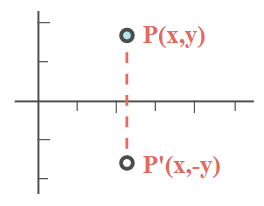
\includegraphics[width = 0.3\textwidth]{Images/Capítulo 4/simetriaX.png}} \hspace{0.5cm}
        \subfloat[Simetría respecto del eje de ordenadas.]{
            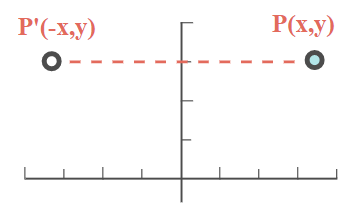
\includegraphics[width = 0.3\textwidth]{Images/Capítulo 4/simetriaY.png}} \vspace{10mm}
        \subfloat[Simetría de un objeto respecto de un eje cualquiera.]{
            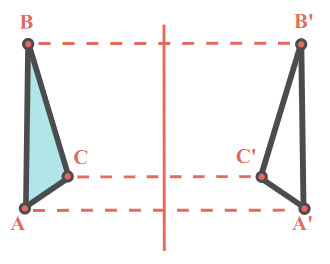
\includegraphics[width = 0.4\textwidth]{Images/Capítulo 4/simetria.png}}
        \caption{Simetrías de forma gráfica. Imagen de \cite{sangaku}}
        \end{figure}
\end{itemize}
Una vez entendidas las definiciones de estas transformaciones se dan ejemplos de composiciones musicales en las que aparecen.
\begin{itemize}
    \item \textbf{Traslaciones}. En la Música, este tipo de transformación se puede entender de dos formas distintas:
    \begin{enumerate}
        \item \textit{Traslación} de una estructura musical. Un canon, tal y como está definido, es una forma de composición en la que una voz interpreta una melodía y, a continuación, a una cierta distancia de compases, otras voces interpretan esa misma melodía. Es decir, la misma partitura que interpreta un instrumento, lo hace otro pero a una distancia en el tiempo:
        \begin{table}[H]
            \centering
            \begin{tabular}{c|c|c|c|c|c}
                Primera voz $\rightarrow$ & A & B & C & D & \cdots \\
                \hline
                Segunda voz $\rightarrow$ &   & A & B & C & \cdots \\
                \hline
                Tercera voz $\rightarrow$ &   &   & A & B & \cdots \\
                \hline
                Cuarta voz  $\rightarrow$ &   &   &   & A &  \cdots \\
                \hline
            \end{tabular}
            \caption{Estructura de canon.}
        \end{table}
        En la tabla se puede observar lo explicado en el párrafo anterior: la primera voz interpreta una melodía y, en este caso, una vez terminado el compás A, la segunda voz comienza a interpretar esa misma melodía, y así sucesivamente con el resto de las voces. Por lo tanto, la estructura de canon es una \textit{traslación} de toda la partitura.
        \item \textit{Traslación} de una motivo en el tiempo. Es decir, un fragmento de una melodía es repetido recursivamente a lo largo de la obra. Por ejemplo, en el Canon de Pachelbel, la voz grave (normalmente interpretada por el Cello) repite durante toda la obra las mismo 8 notas:
        \begin{figure}[H]
            \centering
            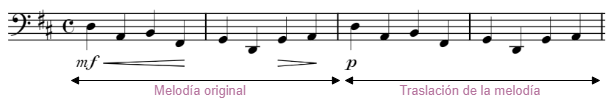
\includegraphics[width = 0.9\textwidth]{Images/Capítulo 4/canonCello.png}
            \caption{Traslación de una melodía en el tiempo.}
        \end{figure}
    \end{enumerate}
    \item \textit{Rotación} de una melodía. Las rotaciones en Música solo tienen sentido si el ángulo $\alpha$ es de $180º$ ya que, en otro caso, no se podría leer la partitura. Sabiendo esto, al igual que en el caso de las traslaciones, hay dos formas de entender esta transformación en Música:
    \begin{itemize}
        \item \textit{Rotación} en un compás o pentagrama. En la siguiente figura se puede ver un compás al que se le ha aplicado una rotación de ángulo $\alpha = 180º$ y de centro el punto rojo P.
        \begin{figure}[H]
            \centering
            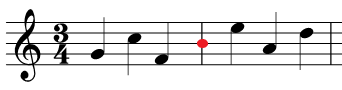
\includegraphics[width = 0.35\textwidth]{Images/Capítulo 4/rotacionPartitura.png}
            \caption{Rotación de un compás 180º.}
        \end{figure}
        Tal y como se explica en \cite{santa} (Santamaría, 2009), otra forma de realizar una rotación a un compás o pentagrama es, a partir de un conjunto de notas escritas de izquierda a derecha, bajar la tonalidad de todas ellas una octava y reescribirlas en la partitura variando el orden: de derecha a izquierda. Gráficamente se tiene:
        \begin{figure}[H]
            \centering
            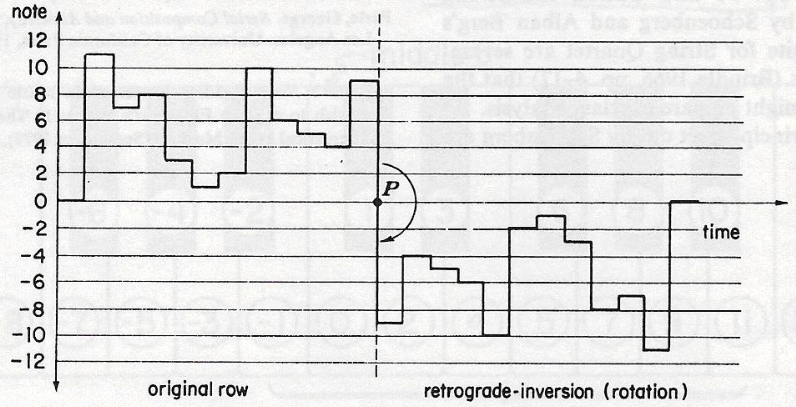
\includegraphics[width = 0.6\textwidth]{Images/Capítulo 4/rotacionGrafica.png}
            \caption{Rotación de forma gráfica. \cite{santa}}
        \end{figure}
        
        \item \textit{Rotación} de la partitura. Otra forma de aplicar rotaciones a una composición musical es girar la partitura completa. Se tiene un ejemplo muy concreto de este tipo de transformación: ``El dueto del espejo''. Esta es una composición atribuida a Mozart en la que dos violines interpretan la misma partitura pero, mientras uno de ellos lo hace en sentido normal: de arriba abajo, el otro recorre la partitura en sentido contrario. Es decir, un intérprete comienza por el primer compás y el otro por el último, se cruzan a la mitad y cada uno termina donde comenzó el otro. A continuación, se muestran los primeros compases leídos tanto desde arriba como desde abajo. Se comprueba que ambos instrumentos tocan las mismas notas, pero en distinta octava. Se puede ver la partitura completa en el Apéndice B.
        \begin{figure}[H]
            \centering
            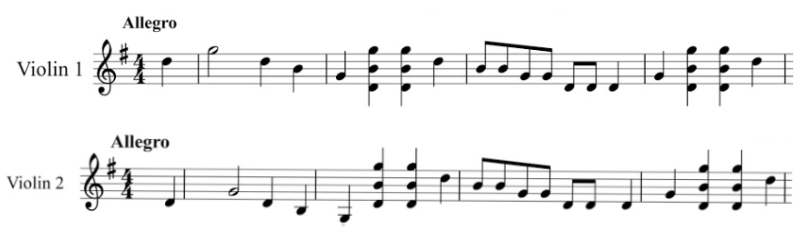
\includegraphics[width = 0.8\textwidth]{Images/Capítulo 4/dueto1.png}
            \caption{Primeros compases ``Dueto del espejo''.}
        \end{figure}
        % \begin{figure}[H]
        %     \centering
        %     \includegraphics{}
        %     \caption{Primeros compases "Dueto del espejo". Sentido contrario.}
        % \end{figure}
    \end{itemize}
    \item \textit{Simetría}. Al igual que en el plano, la simetría puede ocurrir respecto a un eje horizontal o respecto a uno vertical. 
    \begin{itemize}
        \item \textit{Simetría respecto de un eje horizontal}. En este caso, al ser un eje horizontal, las notas simétricas aparecerán escritas por debajo o por encima de las originales obteniendo acordes. 
        \begin{figure}[H]
            \centering
            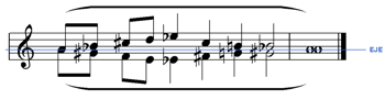
\includegraphics[width = 0.6\textwidth]{Images/Capítulo 4/simetriahorizontal.png}
            \caption{Ejemplo de acordes en simetría.}
        \end{figure}
        En este tipo de simetría se verifica que si se marcan las teclas del piano que se corresponden con los acordes, la figura que se obtiene también es simétrica.:
        \begin{figure}[H]
            \centering
            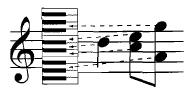
\includegraphics[width = 0.3\textwidth]{Images/Capítulo 4/simetriapiano.png}
            \caption{Simetría horizontal en las teclas del piano. \cite{arbones}}
        \end{figure}
        Sin embargo, muchos compositores utilizan la simetría en un eje horizontal junto con la traslación. Es decir, aparecen escritas las notas simétricas respecto de un eje horizontal pero en compases más avanzados. Por ejemplo, en la Fuga 6, en Re menor, del \textit{Clave bien temperado} de Johann Sebastian Bach aparecen los siguientes compases que representan la simetría que se acaba de explicar. 
        \begin{figure}[H]
            \centering
            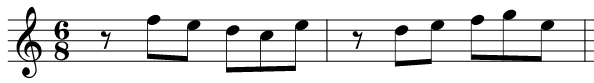
\includegraphics[width = 0.6\textwidth]{Images/Capítulo 4/simetriaTraslacionFuga.png}
            \caption{Ejemplo de simetría y traslación. Fuga 6 de Johann Sebastian Bach.}
        \end{figure}
        \item \textit{Simetría respecto de un eje vertical}. En este caso, el eje de simetría puede estar en la barra de separación de un compás, o en una nota:
        \begin{figure}[H]
        \centering
        \subfloat[Simetría vertical con el eje en una nota. \cite{santa}]{
            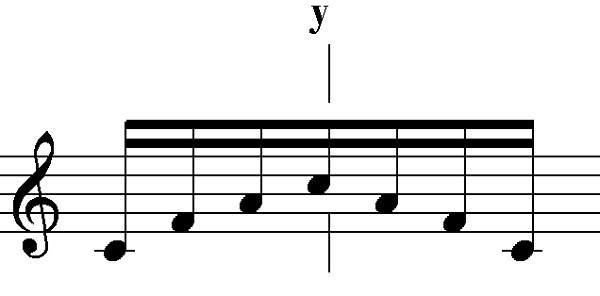
\includegraphics[width = 0.3\textwidth]{Images/Capítulo 4/simetriaPartitura.png}} \hspace{0.5cm}
        \subfloat[Simetría vertical con el eje en una barra de separación.]{
            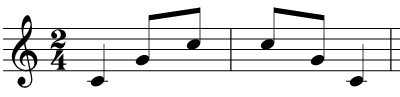
\includegraphics[width = 0.3\textwidth]{Images/Capítulo 4/simetriaBarra.png}} 
        \caption{Simetrías respecto de un eje vertical.}
        \end{figure}
        Un ejemplo real en composición es el <<Aleluya>> del oratorio \textit{El Mesías} de Georg Friedrich Händel, donde aparece una simetría respecto de un eje vertical ubicado en una nota.
        \begin{figure}[H]
            \centering
            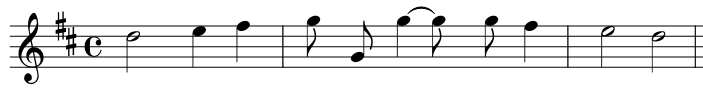
\includegraphics[width = 0.6\textwidth]{Images/Capítulo 4/simetriaHandel.png}
            \caption{Ejemplo simetría vertical. \textit{El Mesías}, Händel.}
            \label{aleluya}
        \end{figure}
        En este caso, la duración de las notas no es simétrica, sin embargo si se tiene en cuenta únicamente la armonía se comprueba que, efectivamente, es una melodía simétrica.
        \begin{figure}[H]
            \centering
            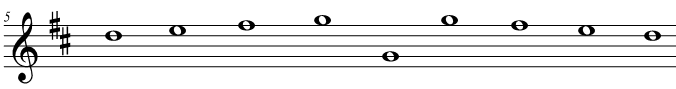
\includegraphics[width = 0.6\textwidth]{Images/Capítulo 4/simetriaHandel2.png}
            \caption{Ejemplo simetría vertical.}
        \end{figure}       
    \end{itemize}
\end{itemize}
Con todos los ejemplos anteriores descritos en este epígrafe, se ha intentado hacer patente que existen composiciones musicales en las que se utiliza algún tipo de transformación geométrica.
    
\chapter{Pulso, tempo y compás}
Otro aspecto en el que se relaciona la Música con las Matemáticas es en la forma de organizar los compases dentro de una partitura. Se va a ver a continuación que la estructura rítmica del sistema musical actual está basada en números. Nada más comenzar a leer una partitura se tiene la clave musical y unos números:
\begin{figure}[H]
    \centering
    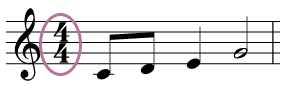
\includegraphics[width = 0.3\textwidth]{Images/Capítulo 5/compas.png}
    \caption{Comienzo de una partitura.}
\end{figure}
Para poder comprender esta notación es importante primero entender los conceptos de \textit{ritmo musical}, \textit{pulso} y \textit{tempo}.\\\\
Según la RAE, se define ritmo como \textit{``la proporción guardada entre los acentos, pausas y repeticiones de diversa duración en una composición musical''}. De forma más intuitiva, se habla de \textit{ritmo musical} cuando los sonidos se suceden de una forma regular y recurrente, pudiendo diferenciar entre elementos fuertes y débiles.\\
Se particulariza este concepto con el adjetivo \textit{``musical''} porque el ritmo subyace en otras formas del arte como la poesía o la danza.\\\\
Ahora bien, aquello que se repite en el ritmo se denomina \textit{pulso}. Tal y como describe Javier Arbonés (2012, p. 37 \cite{arbones}):\\
\textit{``Al oír Música surge en el oyente la necesidad de acompañar ciertas articulaciones con movimientos de un pie, de una mano o de la cabeza. Esta primera agrupación rítmica percibida es lo que se denomina <<pulso>>''.}\\\\
A la hora de generar pulsos, existen distintos patrones de repetición pudiendo, por ejemplo, acentuar la primera nota de cada dos:
\begin{table}[H]
    \centering
    \begin{tabular}{|c|c|c|c|c|c|c|c|c|}
    \hline
        \cellcolor{acento}1 & 2 & \cellcolor{acento}1 & 2 & \cellcolor{acento}1 & 2 & \cellcolor{acento}1 & 2 & $\cdots$ \\
    \hline
    \end{tabular}
\end{table}
O la primera de cada tres:
\begin{table}[H]
    \centering
    \begin{tabular}{|c|c|c|c|c|c|c|c|c|c|c|c|c|}
    \hline
        \cellcolor{acento}1 & 2 & 3 & \cellcolor{acento}1 & 2 & 3 & \cellcolor{acento}1 & 2 & 3 & \cellcolor{acento}1 & 2 & 3 & $\cdots$ \\
    \hline
    \end{tabular}
\end{table}
Y por último, la primera de cada cuatro:
\begin{table}[H]
    \centering
    \begin{tabular}{|c|c|c|c|c|c|c|c|c|c|c|c|c|c|c|c|c|}
    \hline
        \cellcolor{acento}1 & 2 & 3 & 4 & \cellcolor{acento}1 & 2 & 3 & 4 & \cellcolor{acento}1 & 2 & 3 & 4 & \cellcolor{acento}1 & 2 & 3 & 4 & $\cdots$ \\
    \hline
    \end{tabular}
\end{table}
A cada una de estas agrupaciones, formada por el pulso acentuado y los pulsos débiles que vienen después, se le denomina \textit{compás}:
\begin{figure}[H]
    \centering
    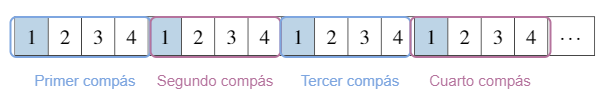
\includegraphics[width = 0.8\textwidth]{Images/Capítulo 5/compases.png}
    \caption{Compás dividido en cuatro pulsos.}
\end{figure}
El \textit{pulso} es, por tanto, el ``latido'' de la pieza musical. De hecho, se mide igual que el latido cardiaco: en latidos por minuto. Esto también viene indicado al inicio de las partituras:
\begin{figure}[H]
    \centering
    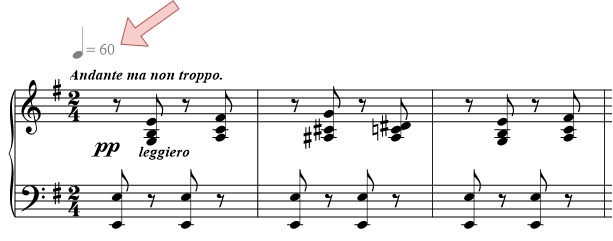
\includegraphics[width = 0.7\textwidth]{Images/Capítulo 5/tempo2.png}
    \caption{Indicación en partitura de los pulsos por minuto.}
\end{figure}
En este caso, por ejemplo, son 60 latidos por minuto: en un minuto se habrán interpretado 60 pulsos, uno por segundo.\\\\
Este número, por tanto, indica la velocidad del pulso, y eso se conoce en Música como \textit{tempo}.\\ En muchos casos, el \textit{tempo} no viene definido con números, sino con palabras, algunas de ellas muy conocidas, como ``Allegro'', ``Andante'', ``Vivace'', etc.
\begin{table}[H]
    \centering
    \begin{tabular}{c|c}
     Pulso por minuto & \textit{tempo} \\
    \hline \hline
     40 - 43 & Grave\\
     44 - 47 & Largo \\
     48 -51 & Larghetto \\
     52 - 54 & Adagio\\
     55 - 65 & Andante \\
     66 - 69 & Andantino \\
     70 - 95 & Moderato \\
     96 - 112 & Allegretto \\
     113 - 120 & Allegro \\
     121 - 140 & Vivace \\
     141 - 175 & Presto\\
     176 - 208 & Prestissimo\\
     \hline
    \end{tabular}
    \caption{Pulsos por minuto y \textit{tempo}.}
\end{table}

Esta primera agrupación rítmica que se ha definido como \textit{pulso} se puede descomponer obteniendo, de esta forma, un ritmo interno que se denomina \textit{``subdivisión del pulso''}. El ritmo interno puede ser binario, cuando el pulso se subdivide en dos, o ternario cuando se subdivide en tres, como ocurre por ejemplo en los valses.\\
De esta forma, se obtienen diversos ritmos pudiendo ser:
\begin{itemize}
    \item Ritmos donde se acentúa la primera de cada dos y cada pulso se subdivide en dos:
    \begin{table}[H]
    \centering
    \begin{tabular}{|c|c|c|c|c|c|c|c|c|c|c|c|c|c|c|c|}
    \hline
        \multicolumn{2}{|c}{\cellcolor{acento}1} & \multicolumn{2}{|c}{2} & \multicolumn{2}{|c}{\cellcolor{acento}1} & \multicolumn{2}{|c}{2} & \multicolumn{2}{|c}{\cellcolor{acento}1} & \multicolumn{2}{|c}{2} & \multicolumn{2}{|c}{\cellcolor{acento}1} & \multicolumn{2}{|c|}{2} \\
        \hline
        \cellcolor{acento}1 & 2 & 1 & 2 & \cellcolor{acento}1 & 2 & 1 & 2 & \cellcolor{acento}1 & 2 & 1 & 2 & \cellcolor{acento}1 & 2 & 1 & 2\\
        \hline
    \end{tabular}
\end{table}
    \item Ritmos donde se acentúa la primera de cada dos y cada pulso se subdivide en tres:
    \begin{table}[H]
    \centering
    \begin{tabular}{|c|c|c|c|c|c|c|c|c|c|c|c|c|c|c|c|c|c|c|c|c|c|c|c|}
    \hline
        \multicolumn{3}{|c}{\cellcolor{acento}1} & \multicolumn{3}{|c}{2} & \multicolumn{3}{|c}{\cellcolor{acento}1} & \multicolumn{3}{|c}{2} & \multicolumn{3}{|c}{\cellcolor{acento}1} & \multicolumn{3}{|c}{2} & \multicolumn{3}{|c}{\cellcolor{acento}1} & \multicolumn{3}{|c|}{2} \\
        \hline
        \cellcolor{acento}1 & 2 & 3 & 1 & 2 & 3 & \cellcolor{acento}1 & 2 & 3 & 1 & 2 & 3 & \cellcolor{acento}1 & 2 & 3 & 1 & 2 & 3 & \cellcolor{acento}1 & 2 & 3 & 1 & 2 & 3 \\
        \hline
    \end{tabular}
\end{table}
    \item Ritmos donde se acentúa la primera de cada tres y cada pulso se subdivide en dos:
    \begin{table}[H]
    \centering
    \begin{tabular}{|c|c|c|c|c|c|c|c|c|c|c|c|c|c|c|c|c|c|c|c|c|c|c|c|}
    \hline
        \multicolumn{2}{|c}{\cellcolor{acento}1} & \multicolumn{2}{|c}{2} & \multicolumn{2}{|c}{3} & \multicolumn{2}{|c}{\cellcolor{acento}1} & \multicolumn{2}{|c}{2} & \multicolumn{2}{|c}{3} & \multicolumn{2}{|c}{\cellcolor{acento}1} & \multicolumn{2}{|c}{2} & \multicolumn{2}{|c}{3} & \multicolumn{2}{|c}{\cellcolor{acento}1} & \multicolumn{2}{|c}{2} & \multicolumn{2}{|c|}{3} \\
    \hline
        \cellcolor{acento}1 & 2 & 1 & 2 & 1 & 2 & \cellcolor{acento}1 & 2 & 1 & 2 & 1 & 2 & \cellcolor{acento}1 & 2 & 1 & 2 & 1 & 2 & \cellcolor{acento}1 & 2 & 1 & 2 & 1 & 2\\
        \hline
    \end{tabular}
\end{table}
\item De este modo, se pueden realizar el resto de combinaciones obteniendo diversos patrones tanto binarios como ternarios.
\end{itemize}
Volviendo a la forma en la que se ha definido el compás, estas combinaciones anteriormente descritas se transforman en números que, tal y como se ha comenzado diciendo en este apartado, se escriben al inicio de los pentagramas para indicar cómo se mide esa obra. Por tanto, si la subdivisión es binaria y:
\begin{itemize}
    \item el compás tiene dos pulsos, se denomina \textit{dos por cuatro}
    \item el compás tiene tres pulsos, se denomina \textit{tres por cuatro}
    \item el compás tiene cuatro pulsos, se denomina \textit{cuatro por cuatro}
\end{itemize}
 \begin{figure}[H]
        \centering
        \subfloat[Dos por cuatro.]{
            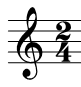
\includegraphics[width = 0.1\textwidth]{Images/Capítulo 5/doscuatro.png}} \hspace{1.7cm}
        \subfloat[Tres por cuatro.]{
            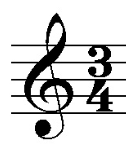
\includegraphics[width = 0.1\textwidth]{Images/Capítulo 5/trescuatro.png}}
            \hspace{1.7cm}
        \subfloat[Cuatro por cuatro.]{
            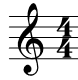
\includegraphics[width = 0.1\textwidth]{Images/Capítulo 5/cuatrocuatro.png}}
            \hspace{1.7cm}
        \caption{Compases binarios.}
        \label{binarios}
\end{figure}
Se observa, entonces, que el numerador en esta ``fracción'' indica el número de pulsos que tiene cada compás pero, ¿qué significa el denominador?\\ 
Para responder a esta pregunta es importante tener en cuenta el valor relativo de las figuras descrito en el Apéndice A: una redonda equivale a dos negras, que a su vez equivalen a cuatro corcheas, etc. Actualmente la nota más larga que se usa es la redonda, por lo que numéricamente la redonda se representa con un 1:
\begin{figure}[H]
    \centering
    \includegraphics[width = 0.7\textwidth]{Images/Capítulo 5/figuras.png}
    \caption{Valor de las figuras teniendo como referencia la redonda.}
    \label{redonda}
\end{figure}
Por tanto, escribir en el pentagrama la ``fracción'' \textit{cuatro por cuatro} (Figura \ref{binarios} (c)), es lo mismo que escribir:
\begin{center}
    \meter{4}{4} = $4 * \frac{1}{4}$ = $4 * $\musQuarter \hspace{0.3cm} $\longrightarrow$ \hspace{0.3cm} cuatro negras por compás
\end{center}
Lo mismo ocurre con el \meter{3}{4} (\textit{tres por cuatro}) y con el \meter{2}{4} (\textit{dos por cuatro}):
\begin{center}
    \meter{3}{4} = $3 * \frac{1}{4}$ = $3 * $\musQuarter \hspace{0.3cm} $\longrightarrow$ \hspace{0.3cm} tres negras por compás\\
    \meter{2}{4} = $2 * \frac{1}{4}$ = $2 * $\musQuarter \hspace{0.3cm} $\longrightarrow$ \hspace{0.3cm} dos negras por compás
\end{center}
En consecuencia, se podría decir que el denominador de esta ``fracción'' no es un valor numérico, sino que es la representación numérica de la figura musical. Sin embargo, la duración de cada figura musical sí que tiene un sentido matemático, de hecho sigue una progresión geométrica de razón $\frac{1}{2}$.\\\\
Por otro lado, si la subdivisión es ternaria, la notación es algo más complicada: 
\begin{itemize}
    \item Si el compás tiene dos pulsos, se denomina \textit{seis por ocho}
    \item Si el compás tiene tres pulsos, se denomina \textit{nueve por ocho}
    \item Si el compás tiene cuatro pulsos, se denomina \textit{doce por ocho}
\end{itemize}
 \begin{figure}[H]
        \centering
        \subfloat[Seis por ocho.]{
            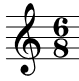
\includegraphics[width = 0.1\textwidth]{Images/Capítulo 5/seisocho.png}} \hspace{1.7cm}
        \subfloat[Nueve por ocho.]{
            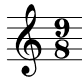
\includegraphics[width = 0.1\textwidth]{Images/Capítulo 5/nueveocho.png}}
            \hspace{1.7cm}
        \subfloat[Doce por ocho.]{
            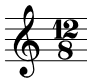
\includegraphics[width = 0.1\textwidth]{Images/Capítulo 5/doceocho.png}}
            \hspace{1.7cm}
        \caption{Compases ternarios.}
\end{figure}
Al igual que en el caso de los compases binarios, el numerador indica el número de pulsos que hay por cada compás y el denominador qué figura musical se toma de referencia. En este caso y tal y como se puede ver en la Figura 19, $\frac{1}{8}$ corresponde a la corchea, es decir:
\begin{center}
    \meter{6}{8} = $6 * \frac{1}{8}$ = $6 * $\musEighth \hspace{0.3cm} $\longrightarrow$ \hspace{0.3cm} seis corcheas por compás\\
    \meter{9}{8} = $9 * \frac{1}{8}$ = $9 * $\musEighth \hspace{0.3cm} $\longrightarrow$ \hspace{0.3cm} nueve corcheas por compás\\
    \meter{12}{8} = $12 * \frac{1}{8}$ = $9 * $\musEighth \hspace{0.3cm} $\longrightarrow$ \hspace{0.3cm} doce corcheas por compás\\
\end{center}
\section{Ritmos Euclidianos}
Una vez explicado cómo el ritmo musical, pulso y los compases están relacionados con las Matemáticas, a continuación se van a utilizar dichos conceptos para desarrollar un tema que, de forma muy concreta, relaciona las dos disciplinas: se trata de los ritmos Euclidianos.\\\\
El algoritmo de Euclides para obtener el \textbf{máximo común divisor} (mcd) de dos números puede ser utilizado para hallar ritmos que son utilizados en la actualidad. Esto fue descubierto por Godfried Toussaint en 2004 y está descrito en un artículo de 2005 \textit{``The Euclidean Algorithm Generates Traditional Musical Rhythms''}. En dicho ensayo, Toussaint explica que, tal y como se aclara en \cite{wikieuclides}, \textit{el máximo común divisor de dos números es utilizado rítmicamente dando el número de pulsos y silencios, generando casi todo los ritmos más importantes de la Música mundial}. \\\\
Esto, que en el presente trabajo se va a utilizar para crear ritmos, en realidad es un problema matemático muy famoso: \\\\
\textit{Dadas n cajas y k objetos, ¿cómo se deben distribuir los objetos en las cajas de la manera más uniforme posible?}\\\\
Este problema ha sido abordado desde muy diferentes disciplinas, por ejemplo en física, con los sistemas de sincronización en los aceleradores de neutrones, tal y como se explica en \cite{ritmos} o en informática gráfica, con el problema de convertir una recta descrita matemáticamente por dos puntos en el plano a una sucesión de píxeles (Sanz y Tur, R., \cite{ritmos2}).\\\\
Para comprender esto y en primer lugar, es importante recordar en qué consiste el cálculo del máximo común divisor y cómo funciona el algoritmo de Euclides.\\\\
Normalmente, en la escuela se enseña a calcular el máximo común divisor de dos números $a$ y $b$, $mcd(a, b)$, hallando los divisores de cada número y escogiendo el común más grande. Por ejemplo: Sea $a = 12$ y $b = 20$, se quiere calcular el $mcd(12,20)$: 
\begin{itemize}
    \item Divisores de 12 $\longrightarrow$ ${1, 2, 3, \boxed{4}, 6, 12}$
    \item Divisores de 20 $\longrightarrow$ ${1, 2, \boxed{4}, 5, 10}$
\end{itemize}
Al observar los divisores, hay que escoger el máximo que tengan en común, en este caso es 4. 
Ahora bien, el algoritmo de Euclides es mucho más útil, sobre todo cuando se trata de números grandes. Este algoritmo se basa en que, al dividir dos números $a$ y $b$, se obtiene un cociente $c$ y un resto $r$, de forma que $a = bc + r$. Euclides demostró que el máximo común divisor de $a$ y $b$ es el mismo que el de $b$ y $r$. 
\begin{teor}
El máximo común divisor de dos números $a$ y $b$, con $a, b \in \mathbb{N}$ y $a>b>0$, coincide con el máximo común divisor de $b$ y $r$, siendo $r$ el resto que se obtiene al dividir $a$ entre $b$.
\end{teor}
\begin{proof}
Sean $d = mcd(a,b)$ y $t = mcd(b,r)$. Se quiere demostrar que $d = t$.\\
Por cómo se ha definido el máximo común divisor, se tiene que $d$ es divisor tanto de $a$ como de $b$, por lo que se puede escribir:
$$a = a_{1}d \hspace{0.5cm}, \hspace{0.5cm} b = b_{1}d \hspace{0.5cm} \text{con} \hspace{0.3cm} a_{1},b_{1} \in \mathbb{N}$$
Ahora bien, por la prueba de la división se tiene que $a = bc + r$, siendo $c$ el cociente de la división. Si se sustituye en esta igualdad $a = a_{1}d$ y $b = b_{1}d$, se tiene: 
$$a_{1}d = b_{1}dc + r \hspace{0.3cm}\Longrightarrow\hspace{0.3cm} r = a_{1}d - b_{1}d = d(a_{1} - b_{1})$$
Por tanto $d$ es un divisor de $r$. Además, se tenía por hipótesis que $d$ también es un divisor de $b$, por lo que debe dividir a su máximo común divisor, es decir, $d$ es un divisor de $mcd(b,r) = t$.\\\\
Por otra parte, $t$ es un divisor tanto de $b$ como de $r$, por ser su máximo común divisor. Por tanto, se puede escribir 
$$b = b_{2}t \hspace{0.4cm} \text{y} \hspace{0.4cm} r = r_{1}t \hspace{0.4cm} \text{con} \hspace{0.3cm} b_{2},r_{1} \in \mathbb{N}$$ Sustituyendo esto en la igualdad $a = bc + r$ se tiene:
$$a = b_{2}t + r_{1}t \hspace{0.3cm} \Longrightarrow \hspace{0.3cm} a = t(b_{2}+r_{1})$$
Por lo que $t$ es un divisor de $a$ y, como también lo era de $b$, es su un divisor de $mcd(a,b) = d$.\\\\
Como se ha demostrado que $d$ es un divisor de $t$ y $t$ es un divisor de $d$, se tiene que $d = t$ y queda demostrado el teorema.
\end{proof}
Demostrado esto, se puede utilizar el algoritmo de Euclides para calcular el máximo común divisor de dos números. El algoritmo funciona como sigue:\\\\
Sean $a, b \in \mathbb{N}$ con $a>b>0$, se definen $c_{i}$ y $r_{i}$ recursivamente mediante las ecuaciones:
\begin{align*}
    a & = bc_{1} + r_{1} \hspace{0.5cm} (0 \leq r_{1} < b)\\
    b & = r_{1}c_{2} + r_{2} \hspace{0.5cm} (0 \leq r_{2} < r_{1})\\
    r_{1} & = r_{2}c_{3} + r_{3} \hspace{0.5cm} (0 \leq r_{3} < r_{2})\\
    &\cdots\\
    r_{k-3} & = r_{k-2}c_{k-1} + r_{k-1} \hspace{0.5cm} (0 \leq r_{k-1} < r_{k-2})\\
    r_{k-2} & = r_{k-1}c_{k} \hspace{0.5cm} (r_{k} = 0)
\end{align*}
Y del teorema recién demostrado se tiene:
$$mcd(a,b) = mcd(b, r_{1}) = mcd(r_{1}, r_{2}) = \cdots = mcd(r_{k-2}, r_{k-1}) = r_{k-1}$$
\begin{ejem}
Se quiere calcular el máximo común divisor de $721$ y $448$ con el algoritmo de Euclides:
\begin{align*}
    721 &= 448 * 1 + 273\\
    448 &= 273*1 + 175\\
    273 &= 175*1 + 98\\
    175 &= 98*1 + 77\\
    98 &= 77*1 + 21\\
    77 &= 21*3 + 14\\
    21 &= 14*1 + \boxed{7}\\
    14 &= 7*2 + 0
\end{align*}
Por tanto, $mcd(721, 448) = 7$.
\end{ejem}

Una vez recordado en qué consiste el algoritmo de Euclides, se puede utilizar para crear ritmos.\\\\
Supóngase que se quieren distribuir equilibradamente $n$ pulsos con acento (que se escribirá con $\bullet$) en $k$ tiempos musicales para crear un ritmo. En un primer momento, para que sea más sencillo, se va a suponer que $n = 4$ y $k = 11$. Es decir, se quieren distribuir 4 pulsos con acento en 11 tiempos musicales de forma regular o equilibrada. Por ejemplo, no serviría la siguiente distribución:
\begin{table}[H]
    \centering
    \begin{tabular}{|c|c|c|c|c|c|c|c|c|c|c|}
    \hline
         & & & & & & & $\bullet$ & $\bullet$ & $\bullet$ & $\bullet$ \\
        \hline
    \end{tabular}
\end{table}
Los pulsos con acento deben estar mezclados de forma equilibrada en las 11 unidades de tiempo. Esto, traducido al algoritmo de Euclides, implica calcular el máximo común divisor de 11 y 4. El primer paso de dicho algoritmo sería:

$$11 = \boxed{4}*2 + \boxed{3}$$
Por tanto, se empareja cada pulso con acento con los tiempos musicales sin acento, obteniendo 4 parejas y 3 pulsos sin acento sueltos:
% \begin{table}[H]
%     \centering
%     \begin{tabular}{|c|c|c|c|c|c|c|c|c|c|c|}
%     \hline
%          & $\bullet$ & & $\bullet$ & & $\bullet$ & & $\bullet$ & & &\\
%         \hline
%     \end{tabular}
% \end{table}
\begin{figure}[H]
    \centering
    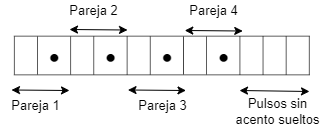
\includegraphics[width = 0.5\textwidth]{Images/Capítulo 5/pulsos.png}
\end{figure}
Repitiendo el proceso, el siguiente paso del algoritmo de Euclides es:
$$4 = \boxed{3}*1 + \boxed{1}$$
Con lo cual, repartiendo de nuevo los espacios vacíos entre las cuatro parejas, se obtienen tres tríos y una pareja suelta:
\begin{table}[H]
    \centering
    \begin{tabular}{|c|c|c|c|c|c|c|c|c|c|c|}
    \hline
         & $\bullet$ & & & $\bullet$ & & &$\bullet$ & & &$\bullet$\\
        \hline
    \end{tabular}
\end{table}
El algoritmo de Euclides seguiría un paso más, sin embargo, de esta forma ya se ha distribuido de manera homogénea los cuatro pulsos entre las once unidades de tiempo.\\\\
Demaine y sus coautores probaron formalmente que este algoritmo proporciona, salvo rotaciones, la única manera de distribuir k objetos entre n cajas del modo más regular posible.(Demaine, \cite{demaine}).\\\\
Este algoritmo tiene las siguientes propiedades:
\begin{enumerate}
    \item Los ritmos euclídeos no cambian al aplicar una rotación. Esto es debido a que lo que importa en este algoritmo es la distancia o intervalo que existe entre cada pulso acentuado, y esto no varía cuando se rota el ritmo. En el ejemplo anterior, las siguientes combinaciones serían correctas y, de hecho, equivalentes a la obtenida:
    \begin{table}[H]
        \centering
        \begin{tabular}{|c|c|c|c|c|c|c|c|c|c|c|}
        \hline
            $\bullet$ & & & $\bullet$ & & & $\bullet$ & & &$\bullet$ &\\
            \hline
        \end{tabular}
        \end{table}

    \begin{table}[H]
        \centering
        \begin{tabular}{|c|c|c|c|c|c|c|c|c|c|c|}
        \hline
            & & $\bullet$ & & & $\bullet$ & & &$\bullet$ & &$\bullet$ \\
            \hline
        \end{tabular}
        \end{table}
    \item Los ritmos euclidianos tienen únicamente dos posibles distancias entre los pulsos con acento:
    \begin{itemize}
        \item La parte entera del cociente $\frac{n}{k}$
        \item La parte entera del cociente $\frac{n}{k}$ más uno.
    \end{itemize}
    En el ejemplo $E(11,4)$, la parte entera de $\frac{11}{4}$ es $2$, por tanto, entre cada pulso con acento solo puede haber una distancia de $2$ o de $3$. Si se observa el patrón dibujado:
    \begin{table}[H]
        \centering
        \begin{tabular}{|c|c|c|c|c|c|c|c|c|c|c|}
        \hline
            $\bullet$ & & & $\bullet$ & & & $\bullet$ & & &$\bullet$ &\\
            \hline
        \end{tabular}
    \end{table}
    Se tiene que los pulsos se encuentran en los espacios 1, 4, 7 y 10, por lo que entre todos ellos hay distancia 3. Entre el pulso que ocupa el lugar décimo y el primero hay distancia 2.
    \item Estos ritmos están compuestos por la repetición de un patrón, llamado patrón principal, y normalmente otro patrón, llamado cola \cite{ritmos} (Gómez, P. \url{http://webpgomez.com/}).\\
    En el ejemplo utilizado anteriormente, el patrón principal es ($\bullet$\hspace{0.1cm} .\hspace{0.1cm} . \hspace{0.1cm}) y la cola es ($\bullet$ \hspace{0.1cm}.\hspace{0.1cm}).\\
    Si $E(k, n)$ es un ritmo euclídeo y $k$ y $n$ no son primos entre sí, entonces la cola es vacía. En caso contrario, la cola no es vacía. Dado que en $E(11,4)$ $k = 11$ y $n = 4$ son primos entre sí, la cola no es vacía. Pero, por ejemplo, si se tiene el ritmo euclidiano $E(12,8)$, se tiene que $k$ y $n$ no son primos entre sí por lo que no tiene cola. De hecho, es de la siguiente forma:
    \begin{table}[H]
        \centering
        \begin{tabular}{|c|c|c|c|c|c|c|c|c|c|c|c|}
        \hline
            & $\bullet$ & $\bullet$ & & $\bullet$ & $\bullet$ & & $\bullet$ & $\bullet$ & &$\bullet$ & $\bullet$\\
            \hline
        \end{tabular}
    \end{table}
    Se puede observar que el patrón principal es (\hspace{0.1cm}. \hspace{0.1cm} $\bullet$ \hspace{0.1cm} $\bullet$) y, curiosamente, se repite 4 veces, que es el máximo común divisor de $12$ y $8$. Como consecuencia se tiene que, en un ritmo euclidiano $E(k,n)$ donde $k$ y $n$ no son primos entre sí y $mcd(k,n) = d$, el patrón principal de E(k,n) se repite exactamente $d$ veces.
\end{enumerate}
Por último, algunos ejemplos de estos ritmos son (Gómez, P. \cite{ritmos}):
\begin{table}[H]
    \centering
    \begin{tabular}{|c|c|}
    \hline
      Ritmo   &  Nombre\\
      \hline \hline
      $E(5,8)$ & Cinquillo cubano, \textit{malfuf} de Egipto, ritmo coreano \textit{mong P'yon}.\\
      \hline
      $E(5,12)$ & Ritmo común en África central.\\
      \hline
      $E(8,3)$ & Son cubano.\\
      \hline
      $E(5, 16)$ & Bossa nova de Brasil.\\
      \hline
    \end{tabular}
    \caption{Ejemplos de ritmos euclidianos.}
\end{table}
\chapter{Actividades para el aula.}
Tal y como se ha mencionado en la introducción, se presentan en este capítulo algunas actividades diseñadas para poder aplicar la teoría desarrollada hasta este momento en el aula. Concretamente, en una clase de 1º de Bachillerato.\\
El objetivo principal es convencer a los alumnos de este curso de la relación que existe entre las Matemáticas y la Música, así como impartir la asignatura de Matemáticas de una forma distinta y original. Para ello, algunas de estas actividades que se desarrollan a continuación utilizan metodologías modernas distintas de la clase tradicional. \\
Se busca de esta manera, fomentar el trabajo en grupo y el aprendizaje cooperativo, crear ambientes donde los alumnos estén cómodos y aprendan de una forma innovadora y promover la utilización de las TIC.\\\\
Algo importante a tener en cuenta es el orden en el que se desarrollará el currículo pues en estas actividades se detallan algunos conceptos musicales que son necesarios para actividades posteriores.\\
El currículo de 1º de Bachillerato está dividido en 5 bloques según el RD 1105/2014, de 26 de diciembre (BOE, \cite{boe}):
\begin{itemize}
    \item Procesos, métodos y actitudes Matemáticas.
    \item Números y Álgebra.
    \item Análisis.
    \item Geometría.
    \item Estadística y Probabilidad.
\end{itemize}
El primer bloque se basa en la planificación del proceso de resolución de problemas, estrategias y procedimientos matemáticos. Se asume que se explica durante todo el curso, por lo que no se ha desarrollado ninguna actividad específica para esta parte, pudiendo desarrollar las competencias que se exigen en ella durante las actividades descritas a continuación. En la siguiente tabla se muestra un esquema de dichas actividades:
\begin{table}[H]
    \centering
    \begin{tabular}{|c|c|}
    \hline
      Bloque & Nombre de la actividad \\
      \hline \hline
      \multirow{2}{*}{Números y Álgebra} & Figuras musicales con números. Figuras con ``puntillo''. \\ 
      \cline{2-2}
      & Método de Euclides. Ritmos Euclidianos. \\
      \hline
      \multirow{2}{*}{Geometría} & Traslaciones, rotaciones y simetrías musicales. \\
      \cline{2-2}
      & Música fractal. \\
      \hline
      Análisis & La función melodía.\\
      \hline
      Probabilidad y Estadística & El juego de los dados de Mozart.\\
      \hline
    \end{tabular}
    \caption{Esquema de actividades.}
\end{table}

\section{Bloque 2: Números y Álgebra.}
\begin{itemize}
    \item \textbf{Actividad I. Figuras musicales con números. Figuras con ``puntillo''.}\\\\
    Se ha diseñado esta actividad con el fin de que los alumnos recuerden las figuras musicales y sus respectivas duraciones y, en concreto, el significado del \textit{puntillo} que en algunas ocasiones se escribe detrás de estas figuras en una partitura.\\
   Obviamente, es primordial que los alumnos conozcan las figuras musicales y, en consecuencia, el profesor deberá iniciar la clase dando una breve explicación de este concepto. Para ello, se puede ayudar de la figura \ref{redonda} o de las figuras \ref{relativo} y \ref{silencios} del Apéndice A. Se tendrá en cuenta, durante toda la actividad, que la redonda dura cuatro pulsos de compás.\\\\
    El \textit{puntillo} que se escribe detrás de una figura musical aumenta la duración un medio de su duración original. Es decir, si se tiene una negra con puntillo, $\musQuarterDotted$, dado que $\musQuarter$ dura un pulso, $\musQuarterDotted$ durará un pulso y medio. De forma numérica: $$\musQuarterDotted = 1 + \frac{1}{2} = \frac{3}{2}$$
    Si se tiene, por ejemplo, una semicorchea con puntillo: $\musSixteenthDotted$, su duración será: $$\musSixteenthDotted = \frac{1}{4} + \frac{1}{8} = \frac{1}{4}(1 + \frac{1}{2}) = \frac{1}{4}\cdot\frac{3}{2}$$
    Realizando más comprobaciones, se observa que el \textit{puntillo} multiplica la duración original de la figura por $\frac{3}{2}$.\\\\
    Si se tiene un segundo \textit{puntillo}, $\quarterNoteDottedDouble$, este aumenta la duración un cuarto de la duración original de la figura (además de la duración extra del primer puntillo). Es decir, una negra con doble \textit{puntillo} $\quarterNoteDottedDouble$ tiene una duración:
    $$1 + \frac{1}{2} + \frac{1}{4} = \boxed{\frac{7}{4}}$$
    Y, de la misma forma, una semicorchea con dos \textit{puntillos}, $\sixteenthNoteDottedDouble$: $$\sixteenthNoteDottedDouble = \frac{1}{4} + \frac{1}{8} + \frac{1}{16} = \frac{1}{4}(1+\frac{1}{2} + \frac{1}{4}) = \frac{1}{4}\cdot\frac{7}{4}$$
    Al igual que en el caso de un solo \textit{puntillo}, si se realizan más comprobaciones, se observa que al añadir dos \textit{puntillos}, la duración de la figura original se multiplica por $\frac{7}{4}$.\\\\
    Es muy raro encontrar partituras en las que se usen más de dos \textit{puntillos}, sin embargo, para llevar a cabo esta demostración se supondrá que se pueden poner tantos como se desee. Se quiere, por tanto, probar que la duración de una figura musical $d_{p}$, donde $d$ es la duración concreta de esa figura y $p$ el número de puntillos que le acompañan, es: $$d_{p} = d[2-(\frac{1}{2})^{p}]$$
    Se dice que es una demostración deductiva porque, a partir de las comprobaciones realizadas anteriormente, se \textit{deduce} que la duración de una figura con $p$ \textit{puntillos} se puede escribir de la forma: $$d_{p} = d(1 + \frac{1}{2} + \frac{1}{2^{2}} + \cdots + \frac{1}{2^{p}}) = d\sum_{i=0}^{p}(\frac{1}{2})^{i}$$
    Dado que esto es una serie geométrica, se necesita conocer este concepto así como la forma de calcular la suma. Esto último se puede mandar como deberes a los alumnos:
    \begin{teor}
    Dada la suma de una serie geométrica $L$ de la forma: 
    $$L = 1 + r + r^{2} + r^{3} + \cdots + r^{m}$$
    Se tiene que
    $$\sum_{i=0}^{m}r^{i} = \frac{1-r^{m+1}}{1-r}$$
    \end{teor}
    \begin{proof}
    \begin{eqnarray*}
    L & = & 1 + r + r^{2} + r^{3} + \cdots + r^{m} = r(\frac{1}{r} + 1 + r + r^{2} + r^{3} + \cdots + r^{m-1}) = \\
    & = & r(\frac{1}{r} + L - r^{m}) = 1 + L\cdot r - r^{m+1}  \Longrightarrow L - L\cdot r = 1 - r^{m+1} \\
    & \Longrightarrow & L(1-r) = 1-r^{m+1} \Longrightarrow \boxed{L = \frac{1-r^{m+1}}{1-r}}
    \end{eqnarray*}
    \end{proof}
    Con lo cual, se tiene que:
    \begin{eqnarray*}
    d\sum_{i=0}^{p}(\frac{1}{2})^{i} & = & d\left[\frac{1-(\frac{1}{2})^{m+1}}{1-\frac{1}{2}}\right] \\
    & = & d[2(1-(\frac{1}{2})^{m+1})] = \boxed{d(2-(\frac{1}{2})^{m})}
    \end{eqnarray*}
    Por tanto, queda demostrado que una figura musical de duración $d$ seguida de $m$ \textit{puntillos} tiene una duración total de $$d_{m} = d(2-(\frac{1}{2})^{m})$$
    \textbf{Desarrollo de la actividad.}\\\\
    Esta actividad tendrá una duración de una sesión lectiva. Se puede realizar en cualquier momento del bloque de números y álgebra dado que los únicos conceptos matemáticos importantes que se requieren son los correspondientes a las series geométricas, algo que los alumnos de 1º de Bachillerato conocen de cursos anteriores (currículo oficial de 3º ESO). Esta actividad, por tanto, les servirá para repasar conceptos y comprobar que se pueden aplicar en distintos campos. \\
    También les servirá para entender nuevos símbolos matemáticos como puede ser el sumatorio y, sobre todo, para aprender a realizar demostraciones por deducción.\\\\
    La metodología que se plantea en este ejemplo es expositiva, pudiendo además hacer uso de distintos recursos, como un proyector o una pizarra interactiva, con el fin de enseñar a los alumnos distintos ejemplos musicales donde se puedan ver directamente las figuras y los \textit{puntillos}. \\\\
    Como ya se ha dicho, la clase debe comenzar con la explicación de las figuras musicales y del significado del \textit{puntillo}. Una vez se tengan claras estas ideas, se realizarán las deducciones ya descritas sobre cuánto duran las distintas figuras con \textit{puntillo} y se procederá a realizar la demostración expuesta en los párrafos anteriores.\\\\
    Como parte práctica de la actividad, se propone realizar comprobaciones con la fórmula recién demostrada. Por ejemplo: ¿Cuánto dura una fusa con dos \textit{puntillos}?\\
    Utilizando la fórmula se tiene:
    $$\demisemiquaverDottedDouble = \frac{1}{16}[2-(\frac{1}{2})^{2}] = \frac{1}{16}[2-\frac{1}{4}] = \frac{1}{8} - \frac{1}{64} = \frac{7}{64}$$
    Y al calcularlo de la forma corriente, tal y como se ha realizado en un comienzo:
    $$\demisemiquaverDottedDouble = \frac{1}{16} + \frac{1}{32} + \frac{1}{64} = \frac{4+2+1}{64} = \frac{7}{64}$$
    \item \textbf{Actividad II. Método de Euclides. Ritmos Euclidianos.}\\\\
    No se aportan explicaciones del tema en este apartado dado que se pueden encontrar en el capítulo 5.\\\\
    La finalidad de esta actividad es que los alumnos conozcan el algoritmo de Euclides y aprendan a utilizarlo. Además, y al igual que en todas las actividades que se presentan, se pretende que los alumnos comprenderán la estrecha relación que tienen la Música y las Matemáticas.\\\\
    \textbf{Desarrollo de la actividad.}\\\\
    Se realizará en una única sesión lectiva, una vez se hayan repasado las fracciones algebraicas y el método de cálculo del máximo común divisor con el fin de que los alumnos puedan comprender sin problemas el algoritmo de Euclides y su utilidad.\\\\
    Se sugiere para esta actividad utilizar las TIC como recurso didáctico reproduciendo el siguiente vídeo donde el profesor Eduardo Sáenz de la Universidad de La Rioja explica tanto el algoritmo de Euclides como los ritmos Euclidianos: \url{https://www.youtube.com/watch?v=qxRW5pDT2o4}\\
    Probablemente el profesor necesitará realizar ejemplos del algoritmo para que los alumnos asimilen completamente la información. Una vez comprendan el mecanismo, el profesor realizará un ejemplo en la pizarra de cómo encontrar ritmos euclidianos.\\
    Para terminar la clase, se pueden reproducir en el aula canciones o vídeos donde aparezcan estos ritmos. 
\end{itemize}
\section{Bloque 3: Geometría.}
\begin{itemize}
    \item \textbf{Actividad I. Traslaciones, rotaciones y simetrías musicales.}\\\\
    Al igual que en la actividad anterior, no se aportan explicaciones sobre el tema ya que se pueden encontrar en el Capítulo 4.\\\\
    \textbf{Desarrollo de la actividad.}\\\\
    La actividad tendrá una duración de una sesión lectiva. Se puede realizar tanto al comienzo del tema de vectores, como introducción y repaso de los movimientos en el plano, o al final del tema, una vez los alumnos hayan asimilado los conceptos.\\
    Según la temporalización que se elija, se necesitará más tiempo o menos para introducir el tema y los conceptos. Es importante que los alumnos tengan claro las isometrías para que puedan aportar ideas a la hora de ver estos movimientos en composiciones musicales.\\
    El profesor, con ayuda de un ordenador y un proyector, propondrá distintas composiciones en las que se puedan apreciar las transformaciones. En un primer momento, los alumnos escucharán el fragmento elegido y deberán pensar qué tipo de isometría aparece en esa composición. Se plantea, para este momento, crear un ambiente donde los alumnos puedan debatir entre ellos y aportar diferentes ideas. Después, el profesor proyectará la partitura para mostrar la isometría.\\
    En el sección 4.2 ``Geometría y composición'' se han planteado diversos ejemplos que pueden ser usados en el aula.
    \item \textbf{Actividad II. Música fractal.}\\\\
    Se propone una segunda actividad en el bloque de Geometría: la Música fractal. El objetivo es el de que los alumnos comprendan el término fractal y conozcan diversos aspectos donde son muy útiles, concretamente en la composición musical.\\\\
    Un fractal es un elemento geométrico cuya estructura básica (su apariencia y la manera en la que se distribuye) se repite a diferentes escalas.\\
    Este concepto fue definido por primera vez por el matemático Mandelbrot en 1975. Algunos ejemplos de fractales son:
    \begin{figure}[H]
        \centering
        \subfloat{
            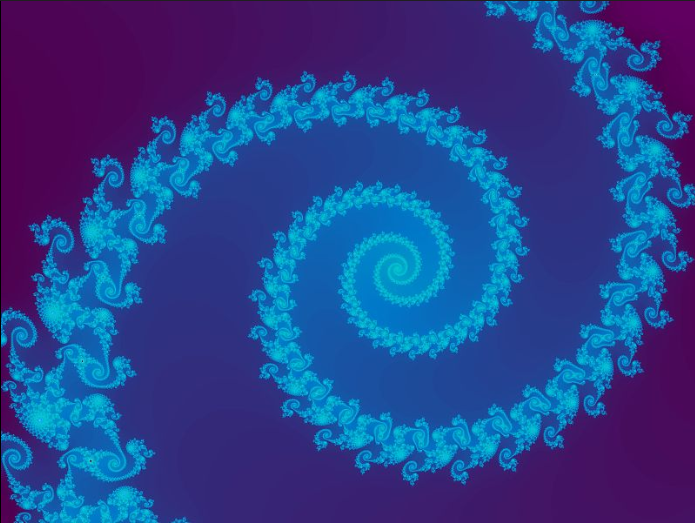
\includegraphics[width = 0.4\textwidth]{Images/Capítulo 6/fractal1.png}} \hspace{1.7cm}
        \subfloat{
            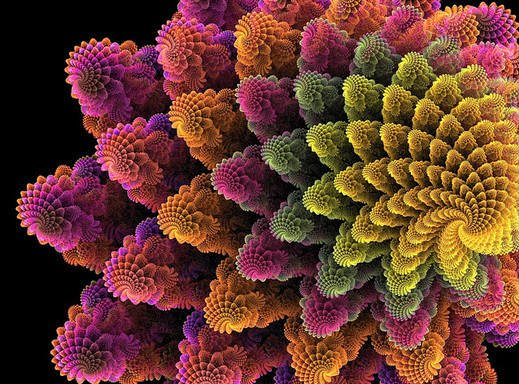
\includegraphics[width = 0.4\textwidth]{Images/Capítulo 6/fractal3.png}}
        \caption{Ejemplos de fractales. \cite{ejemplosfrac}}
    \end{figure}
    Y otros muy famosos son:
    \begin{figure}[H]
        \centering
        \subfloat[Triángulo de Sierpinski]{
            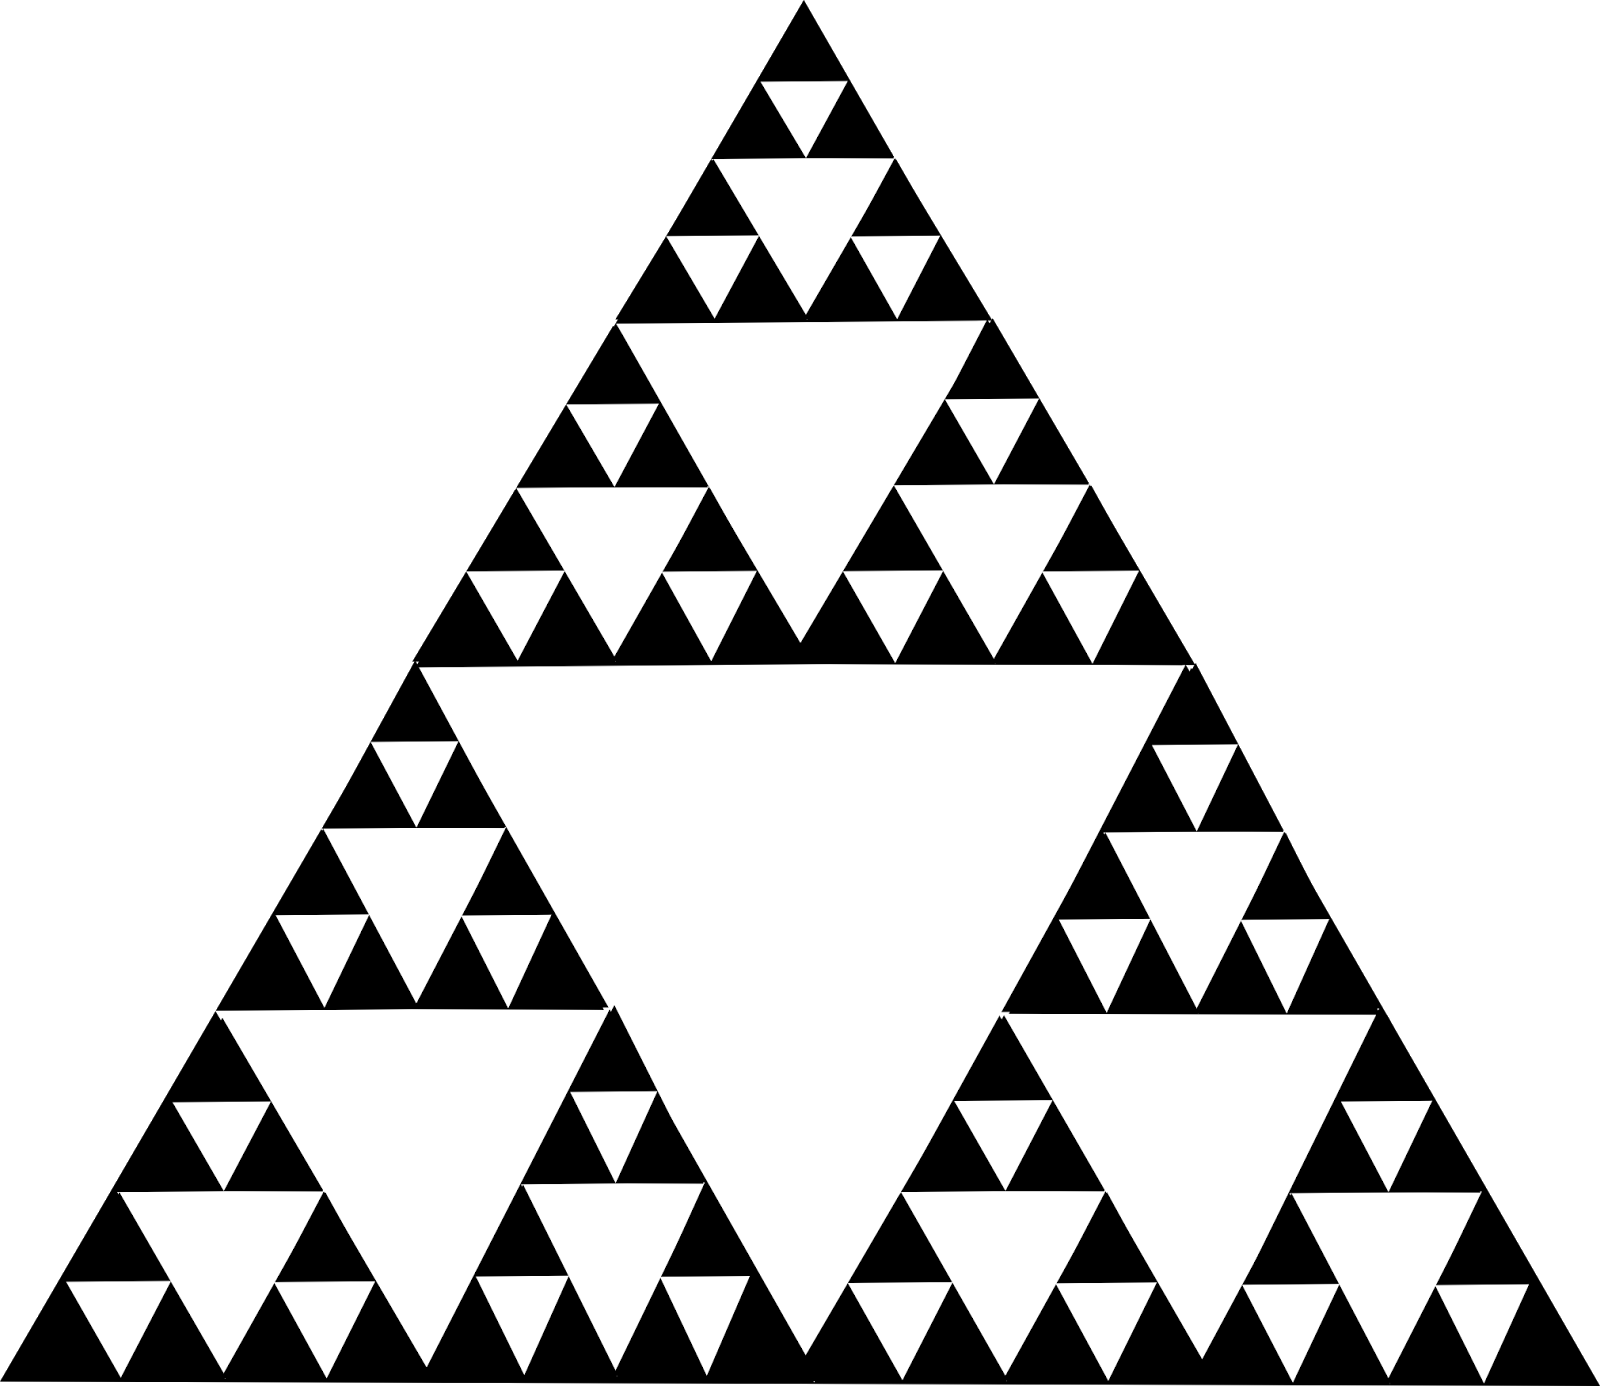
\includegraphics[width = 0.3\textwidth]{Images/Capítulo 6/triangulo.png}} \hspace{1.7cm}
        \subfloat[Copo de nieve de Koch]{
            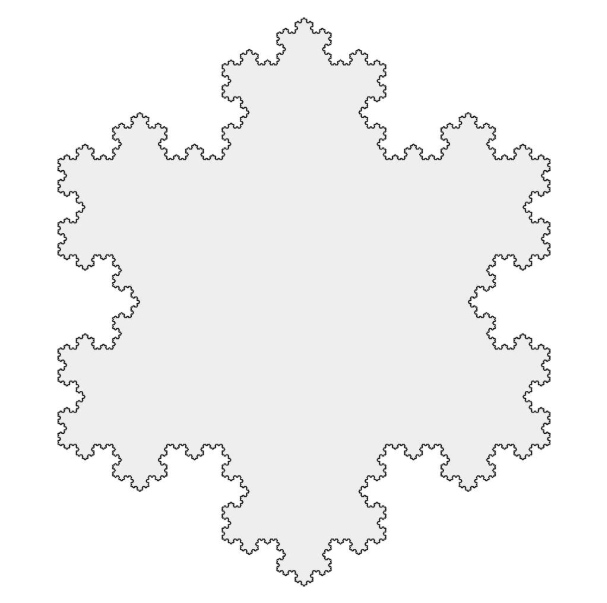
\includegraphics[width = 0.3\textwidth]{Images/Capítulo 6/estrella.png}}
        \caption{Fractales famosos. Imagen de \cite{triangulo}}
    \end{figure}
    Las principales características de estos objetos son:
    \begin{enumerate}
        \item Autosimilaridad. La propia definición de fractal lo indica: su estructura básica no varía si se observa el objeto a diferentes escalas.
        \item La \textit{dimensión fractal}, $d_{f}$, es estrictamente mayor a la \textit{dimensión topológica}, $d_{t}$.
        $$d_{f} > d_{t}$$
        La dimensión, como concepto matemático, se refiere a las propiedades topológicas de una forma u objeto según su capacidad de desarrollo espacial. Por ejemplo, un cuadrado se representa en el espacio en forma de plano, mientras que un cubo es un volumen. Esto, en términos numéricos, se expresa en la \textit{dimensión}, siendo todos los planos de dimensión 2, los volúmenes de dimensión 3 y las rectas de dimensión 1. \cite{dimension}\\
        Por otra parte, la \textit{dimensión fractal} se ha definido durante los últimos años de muchas formas distintas y no todas son equivalentes. Esto se explica de forma más extensa en \cite{fractales} ({Pérez J.A.} (2000), \url{japerez@dlsi.ua.es}).\\
        Básicamente, esta dimensión determina cuánto parece llenar un fractal el espacio conforme se amplía el objeto a escalas más pequeñas.
        \item Los fractales no son diferenciables en ningún punto. Es decir, no gozan de las propiedades de “suavidad” de las funciones derivables.\\
        En la introducción de este capítulo se ha mencionado la necesidad de tener en cuenta el orden de explicación de los bloques ya que hay conceptos que los alumnos deben tener para comprender distintas actividades. En este caso, los alumnos no entenderán el concepto \textit{diferenciable} si antes no se ha explicado el bloque de análisis.\\
        Si esta circunstancia se diera y los alumnos estuvieran familiarizados con las funciones, el profesor puede completar este apartado mostrando a los alumnos una función continua pero no diferenciable en ningún punto. La función de Weierstrass cumple estas condiciones. Weierstrass fue el primer matemático en dar un ejemplo de una función continua en un intervalo, pero no diferenciable en ninguno de sus puntos:
        $$\sigma(x) = \sum_{n=0}^{\infty}a^{n}\cos{b^{n}\pi x}$$
        Weierstrass demostró que si $0<a<1$ y $b$ es un entero positivo e impar y se cumple la condición:
        $$ab>1+\frac{3}{2}\pi$$
        entonces la función $\sigma(x)$ es continua en todo ${\rm I\!R}$ y no es derivable en ningún punto.\\
        Tal y como se aprecia en la siguiente imagen de \cite{weier}, esta función se comporta como un fractal aunque no cumple de forma rigurosa la propiedad de autosimilaridad:
        \begin{figure}[H]
            \centering
            \includegraphics[width = 0.6\textwidth]{Images/Capítulo 6/weierstrass.png}
            \caption{Función de Weierstrass. Imagen de \cite{weier}.}
            \label{fig:my_label}
        \end{figure}
    \end{enumerate}
    Estos objetos se utilizan para estudiar una infinidad de fenómenos, como el comportamiento de los terremotos, los movimientos de la bolsa, compresión de imágenes de ordenador, neurociencia, etc.\\
    Una aplicación concreta en la que se utilizan es, como se ha dicho, en la Música. \\
    Se define Música fractal como \textit{aquella que ha sido generada a partir de la proyección en un espacio musical del comportamiento de un determinado fractal} \cite{fractales} ({Pérez J.A.} (2000), \url{japerez@dlsi.ua.es}). Por lo tanto, en un primer momento se puede pensar que la Música fractal es algo moderno (y el concepto en sí lo es). Y, sin embargo, diferentes estudios han encontrado rasgos de autosemejanza en algunas piezas clásicas, como por ejemplo \textit{La coral} de ``Kunst der Fuge'' de Johann Sebastian Bach, en la que las mismas melodías son repetidas por distintos instrumentos y con distintas variaciones. En concreto, varias voces repiten al doble de velocidad la melodía de la voz principal.\\
    En \cite{fractales} se pueden encontrar muchos más ejemplos de investigaciones que analizan la manifestación de estructuras fractales en composiciones clásicas.\\\\
    Ahora bien, la Música fractal, tal y como se ha definido, se basa en proyectar el comportamiento de un fractal sobre un espacio musical.\\
    Cada vez hay más compositores que utilizan los fractales para crear sus obras. En casi todos los casos, se ayudan de programas informáticos que generan secuencias de sonidos basados en fractales. Por ejemplo, Phil Thompson, basó todas sus composiciones en el conjunto de Mandelbrot, utilizando un programa informático llamado ``Gingerbread'' (V. Hugo, 2014, \cite{gingerbread}.\\\\
    \textbf{Desarrollo de la actividad.}\\\\
    Se realizará en una sola clase, utilizando una metodología expositiva. El profesor desarrollará, en primer lugar, el concepto de fractal y proyectará en la pizarra distintos ejemplos. Además, puede explicar cómo construir los fractales más famosos:
    \begin{figure}[H]
        \centering
        \subfloat[Construcción del triángulo de Sierpinski.]{
            \includegraphics[width = 0.4\textwidth]{Images/Capítulo 6/trianguloConstruccion.png}} \hspace{1.7cm}
        \subfloat[Construcción del copo de nieve de Koch.]{
            \includegraphics[width = 0.4\textwidth]{Images/Capítulo 6/estrellaConstruccion.png}}
        \caption{Construcción de fractales famosos. \cite{triangulo}}
    \end{figure}
\end{itemize}
Para que los alumnos comprendan la gran utilidad que tienen los fractales, es conveniente que el profesor aporte algunos ejemplos de cómo se usan en ciencia, economía, etc. Después, se pasará a explicar el concepto de \textit{Música fractal}. \\
Una cuestión interesante que probablemente los alumnos se planteen es ¿cómo se puede transcribir una imagen (un fractal en este caso) a notación musical?. Existen muchos programas informáticos que realizan esta acción como, por ejemplo, el ya citado \textit{Gingerbread}, o \textit{Venharis}, ambos creaciones del compositor mencionado Phil Thompson. Otros ejemplos pueden ser: \textit{Fractal Harmonies, MusicNum 2.08, Make Prime Music}, etc.\\
El profesor, como parte práctica de la actividad, puede mostrar alguno de estos programas en el aula. \textit{Gingerbread} es de acceso gratuito y es sencillo entender su funcionamiento. Victor Hugo (2014, p.8) lo explica detalladamente en \cite{gingerbread}. De forma resumida, el programa se basa en sonorizar segmentos del Conjunto de Mandelbrot y, mediante instrucciones algorítmicas, transforma los parámetros espaciales de la imagen a parámetros de las tonalidades sonoras.
% \textit{El programa sonoriza segmentos del fractal o cuasi-fractal llamado Conjunto de Mandelbrot, pero también de imágenes en formato jpg. Gingerbread maneja series de instrucciones Matemáticas, instrucciones llamadas algoritmos (por eso se le llama también Música algorítmica) con las que dar tratamiento a los parámetros espaciales de la imagen para adaptarlos a los parámetros de las tonalidades sonoras, logrando una traducción de lo espacial a lo auditivo.}
\section{Bloque 4: Análisis.}
El tema de análisis y, concretamente, las funciones suele ser una parte de la asignatura que a los alumnos les resulta especialmente complicada. Esta actividad se ha pensado para despertar la creatividad en los estudiantes y poner de manifiesto las aplicaciones de esta parte de las Matemáticas a la Música.\\\\
Se quiere hacer ver a los alumnos que las melodías se pueden considerar como funciones y, como tal, tienen dominio, tienen recorrido, se puede estudiar su continuidad, derivabilidad, etc. \\
Dado que, obviamente es necesario que los estudiantes conozcan estos conceptos, la actividad se realizará una vez se hayan explicado y se hayan realizado dibujos de funciones, por lo que el momento más razonable sería al terminar este bloque.\\\\
Sea M la función melodía definida en un intervalo de ${\rm I\!R}$, donde la variable independiente es el tiempo (medido en pulsos) y el conjunto imagen es el conjunto de los sonidos (medido en Herzios). Se quiere estudiar:
\begin{itemize}
    \item Dominio / Recorrido
    \item Continuidad y derivabilidad
    \item Simetrías. ¿Es una función par?
    \item Dibujo de la función
\end{itemize}
Como ejemplo para explicar esto se va a tomar un fragmento del <<Aleluya>> del oratorio \textit{El Mesías} de Georg Friedrich Händel (Figura \ref{aleluya}). Un posible esbozo de la función que representa este fragmento es:
\begin{figure}[H]
    \centering
    \includegraphics[width = 0.7\textwidth]{Images/Capítulo 6/funcion1.png}
    \caption{Esbozo de la función que representa el fragmento del <<Aleluya>>.}
\end{figure}
Por lo tanto, la función que se obtiene es:
\begin{figure}[H]
    \centering
    \includegraphics[width = 0.7\textwidth]{Images/Capítulo 6/funcion2.png}
    \caption{Función del fragmento del <<Aleluya>>.}
    \label{funcion}
\end{figure}
El dominio de la función es el intervalo donde está representada y, como la variable independiente $x$ está medida en pulsos, el dominio es: $[0, 12]$ (12 es el número de pulsos que están representados).\\
El recorrido es algo más complejo de explicar. En la Figura \ref{funcion} parece claro que el recorrido es $[392, 784]$, herzios entre los que la función oscila. Sin embargo, esto no es del todo cierto ya que la melodía, en realidad, no pasa por todas las notas comprendidas en ese intervalo. Por ejemplo, el pico que aparece dibujado va de Sol medio a Sol agudo, pero no se interpretan todas las notas que hay entre estos dos Soles. Esto es algo que se deberá explicar a los alumnos para que lo tengan en cuenta; sin embargo se obviará esta contrariedad para que sea más sencillo representar las funciones.\\\\
La función es continua, no tiene saltos. Musicalmente, la función dejará de ser continua cuando haya silencios en la partitura.\\\\
En cuanto a la derivabilidad, una melodía será derivable cuando sea suave. Esta cualidad es algo subjetiva y en la manera en la que se han unido las notas en la figura anterior cabe pensar que siempre van a ser líneas quebradas, por lo que tendrán picos y por tanto las funciones no serán derivables. Sin embargo, se puede explicar a los alumnos que las líneas que unen cada nota no tienen por qué ser rectas. Se decidirá la forma según la melodía sea más o menos suave y es por esto que se ha definido esta cualidad como subjetiva.\\
En el caso anterior (Figura \ref{funcion}), se ve claramente en el dibujo que la función tiene un pico y, por tanto, no es derivable en todo su dominio. Sin embargo, en el caso de la melodía inicial de la obra \textit{Obertura de 1812} de \textit{Thaikovsky} se tiene una melodía muy suave, sin cambios bruscos de tono. Un posible esbozo de la función sería:
\begin{figure}[H]
    \centering
    \includegraphics[width = 0.7\textwidth]{Images/Capítulo 6/ovSilencios.png}
    \caption{Esbozo de la función que representa el fragmento de <<Obertura 1812>>.}
\end{figure}
Y por tanto, si no se tienen en cuenta los silencios iniciales:
\begin{figure}[H]
    \centering
    \includegraphics[width = 0.6\textwidth]{Images/Capítulo 6/ovBuena.png}
    \caption{Función del fragmento de la <<Obertura 1812>>.}
\end{figure}
Esta función es derivable en todo su dominio. \\\\
\textbf{Desarrollo de la actividad.}\\\\
Se realizará en una única clase y, tal y como se ha mencionado, al finalizar el bloque de Análisis.\\\\
En primer lugar, el profesor explicará cómo las melodías pueden ser vistas como funciones mediante un ejemplo. Se propone no utilizar una metodología expositiva, sino que los alumnos participen aportando ideas de cuáles pueden ser los elementos de esa función, creando de esta forma una clase más dinámica.\\\\
Una vez se haya explicado el ejemplo, los alumnos trabajarán en grupos de cuatro o cinco personas. El profesor elegirá una canción distinta para cada grupo. Deberán ser canciones conocidas por todos para que puedan dibujar la melodía sin necesidad de ver una partitura. Algunos ejemplos pueden ser: ``Cumpleaños Feliz'', ``Noche de Paz'', ``La Cucaracha'', ``Resistiré''. También, cada grupo puede elegir una canción por ellos conocida.\\\\
Los alumnos deberán trabajar en equipo para esbozar una posible función que represente esa melodía y hallar los distintos elementos descritos anteriormente. 
\section{Bloque 5: Probabilidad y Estadística.}
Con la idea de introducir a los alumnos en el mundo de la probabilidad, se propone el ``juego de los dados de Mozart'' como recurso didáctico para la enseñanza-aprendizaje de este campo.\\\\
Mozart, mediante el proceso que se va a explicar a continuación, escribió su obra \textit{Musikalisches Würfelspiel}. Se trata de un vals dividido en dos partes: un minueto y un trío, cada uno de ellos de 8 compases. Sin embargo, gracias al sistema que utilizó Mozart para componer esta obra, se pueden escribir una gran cantidad de valses distintos. Por lo tanto, se puede decir que Mozart no solo compuso una obra si no que, gracias a la probabilidad y el azar, creó un generador de valses.\\\\
El juego de dados se basa en dos tablas: una para los minuetos y otra para los tríos. En ambas, las columnas indican el número de orden del compás y en cada una
de las filas aparece un número entre 2 y 12 que corresponde a los números que se pueden obtener al lanzar dos dados.
En el interior de las tablas se encuentra un repertorio de compases cifrados.
\begin{table}[H]
    \centering
    %\resizebox{10cm}{!}{
    \begin{tabular}{|c|c|c|c|c|c|c|c|c|}
    \hline
    \multicolumn{9}{|c|}{Minueto}\\
    \hline \hline 
         & \textbf{I} & \textbf{II} & \textbf{III} & \textbf{IV} & \textbf{V} & \textbf{VI} & \textbf{VII} & \textbf{VIII}\\
         \hline
         \textbf{2} & 96 & 22 & 141 & 41 & 105 & 122 & 11 & 30\\
         \hline
         \textbf{3} & 32 & 6 & 128 & 63 & 146 & 46 & 134 & 81\\
         \hline
         \textbf{4} & 69 & 95 & 128 & 13 & 153 & 55 & 110 & 24\\
         \hline
         \textbf{5} & 40 & 17 & 113 & 85 & 161 & 2 & 159 & 100\\
         \hline
         \textbf{6} & 148 & 74 & 163 & 45 & 80 & 97 & 36 & 107\\
         \hline
         \textbf{7} & 104 & 157 & 27 & 167 & 154 & 68 & 118 & 91\\
         \hline
         \textbf{8} & 152 & 60 & 171 & 53 & 99 & 133 & 21 & 127\\
         \hline
         \textbf{9} & 119 & 84 & 114 & 50 & 140 & 86 & 169 & 94\\
         \hline
         \textbf{10} & 98 & 142 & 42 & 156 & 75 & 129 & 62 & 123\\
         \hline
         \textbf{11} & 3 & 87 & 165 & 61 & 135 & 47 & 147 & 33\\
         \hline
         \textbf{12} & 54 & 130 & 10 & 103 & 28 & 37 & 106 & 5\\
         \hline
    \end{tabular}
    %}
    \caption{Tabla del ``Juego de dados de Mozart''. Minueto.}
\end{table}
\begin{table}[H]
    \centering
    %\resizebox{15cm}{!}{
    \begin{tabular}{|c|c|c|c|c|c|c|c|c|}
    \hline
    \multicolumn{9}{|c|}{Trío}\\
    \hline \hline 
         & \textbf{IX} & \textbf{X} & \textbf{XI} & \textbf{XII} & \textbf{XIII} & \textbf{XIV} & \textbf{XV} & \textbf{XVI}\\
         \hline
         \textbf{2} & 70 & 121 & 26 & 9 & 112 & 49 & 109 & 14\\
         \hline
         \textbf{3} & 117 & 39 & 126 & 56 & 174 & 18 & 116 & 83\\
         \hline
         \textbf{4} & 66 & 139 & 15 & 132 & 73 & 58 & 145 & 79\\
         \hline
         \textbf{5} & 90 & 176 & 7 & 34 & 67 & 160 & 52 & 170\\
         \hline
         \textbf{6} & 25 & 143 & 64 & 125 & 76 & 136 & 1 & 93\\
         \hline
         \textbf{7} & 138 & 71 & 150 & 29 & 101 & 162 & 23 & 151\\
         \hline
         \textbf{8} & 16 & 155 & 57 & 175 & 43 & 168 & 89 & 172\\
         \hline
         \textbf{9} & 120 & 88 & 48 & 166 & 51 & 115 & 72 & 111\\
         \hline
         \textbf{10} & 65 & 77 & 19 & 82 & 127 & 38 & 149 & 8\\
         \hline
         \textbf{11} & 102 & 4 & 31 & 164 & 144 & 59 & 173 & 78\\
         \hline
         \textbf{12} & 35 & 20 & 108 & 92 & 12 & 124 & 44 & 131\\
         \hline
    \end{tabular}
    %}
    \caption{Tabla del ``Juego de dados de Mozart''. Trío.}
\end{table}

El método funciona porque Mozart creó las tablas con dos peculiaridades:
\begin{enumerate}
    \item Aquellos compases que pertenecen a la misma columna son variaciones sobre una idéntica armonía.
    \item Los compases cifrados cumplen reglas musicales tanto de armonía como de melodía.
\end{enumerate}
\textbf{Desarrollo de la actividad.}\\\\
Se realizará en una única clase y una vez que los alumnos tengan los conceptos básicos de probabilidad asimilados. Se busca que sea una clase dinámica, donde los alumnos intervengan con un aprendizaje significativo ya adquirido con el fin de que sean ellos los protagonistas en el aula.\\\\
Como observación, esta actividad también podría utilizarse al inicio del bloque como motivación para introducir a los alumnos este tema de una forma original. Pero en este caso, tanto la metodología a utilizar como el propio desarrollo de la clase serán diferentes de lo que a continuación se va a exponer.\\\\
En primer lugar, se hablará a los alumnos de Mozart. Se puede iniciar la clase, por ejemplo, preguntando: ``¿Quién puede contarnos algo sobre Mozart?''. Se debe aportar una breve biografía para poner en contexto a los alumnos y así también enriquecer su cultura musical.\\
Se les contará, tal y como se ha explicado al inicio de esta sección, el proceso que siguió Mozart para utilizar el “generador de valses” en la creación de su obra y se les entregará una ficha con las tablas antes descritas y los compases que ideó el gran compositor. (Apéndice D).\\\\
La metodología que se propone en este caso es, durante toda la clase, hacer preguntas para que sean los alumnos quienes respondan en todo momento. Si tienen nociones básicas de probabilidad, no tendrán ninguna dificultad:
\begin{itemize}
    \item ¿Al lanzar dos dados, se tiene la misma probabilidad de obtener como suma un 3 que un 6?
    \item Al lanzar un único dado es obvio que todos los números tienen la misma probabilidad. ¿Qué distribución sigue este experimento? ¿Y al lanzar dos dados, que distribución se tiene?
    \item ¿Cuántos valses se pueden crear con este método?
\end{itemize}
Por último, se puede animar a los alumnos a utilizar este procedimiento para componer ellos mismos un vals. Para ello, se dividirá la clase en grupos de cuatro o cinco alumnos y a cada grupo se les entregará una hoja con un pentagrama y dos dados. De esta forma se fomentará el aprendizaje cooperativo.\\
Durante el proceso de esta actividad grupal, el profesor puede explicar por qué el método funciona tan bien.  

\section{Análisis de las actividades.}
Dado que no ha sido posible poner en práctica estas actividades durante un curso escolar, no se pueden ofrecer resultados cuantitativos obtenidos en la observación del trabajo de los alumnos. Sin embargo, se ha pedido a dos profesionales su opinión con respecto a la relación entre las Matemáticas y la Música y, en concreto, a enseñar dicha relación en el aula. A cada uno de ellos se le preguntaron cuestiones relacionadas con su profesión. Las entrevistas completas se encuentran en el apéndice C.\\\\
El primer profesor, Gabriel Gomila, es musicólogo y pedagogo. Se le preguntó, en relación con este último capítulo, sobre qué le parecía utilizar estas actividades para explicar algunos conceptos básicos de la teoría musical. En toda la entrevista se puede observar la importancia que le da al nexo tan significativo que existe entre las Matemáticas y la Música y el gran paso que supondría realizar actividades interdisciplinares entre estas dos áreas. Además, aporta algunas ideas muy interesantes que podrían ser utilizadas en el aula de Matemáticas.\\
Por otra parte y como músico, destaca la importancia que tiene este campo en muchos otros ámbitos y aclara que la explicación matemática que hay debajo de la Música debería ser utilizada más a menudo para desarrollar nuevos campos científicos como, por ejemplo, la medicina. Se ha querido destacar esto ya que este trabajo puede ser un punto de partida para demostrar a los alumnos la importancia que tiene la aplicación de las Matemáticas en muy diversos campos, algunos de ellos que ni siquiera podrían llegar a imaginar y que, sin embargo, pueden llegar a ser muy importantes.\\\\
El segundo profesional, Eduardo Madirolas, ha sido profesor de Matemáticas durante muchos años en el Centro Integrado de Música de San Lorenzo de El Escorial, por lo que ha impartido esta asignatura a alumnos que en el futuro serían músicos. En la entrevista enumera diversas ocasiones en las que él mismo ha utilizado la Música en el aula. De hecho, una de las actividades que explica ha sido detallada en este trabajo: el uso de los movimientos geométricos en la transposición y transformación musical.\\
Al igual que Gabriel, destaca la importancia de la Música en otros aspectos: \textit{Pienso  que  en  toda  la  actividad  mental  la  Música  es  formativa,  tanto  como  las Matemáticas.  Desarrolla  hábitos  de  estudio,  ayuda  a  organizar  la  mente,  potencia  el pensamiento  lógico,  etc.}\\
Por último, este profesor indica que valorar la base social del alumnado, así como el nivel cultural de las familias, es algo necesario antes de proponerse realizar cualquier actividad y esto es algo que se ha aprendido y estudiado en muchas asignaturas del máster, por lo que será primordial realizar este análisis antes de aplicar este proyecto en un aula.\\\\
Para finalizar este capítulo, se quiere destacar una frase de la entrevista: \textit{lo  más  importante  es  saber  transmitir  que  para  ser  sabios  no  basta  con tener  el  conocimiento  de  un  área,  sino  saber  interpretar  las  relaciones  entre  las  distintas áreas para utilizarlas entre sí y sacarles mayor partido.}


\chapter{Conclusiones y líneas de trabajo futuras.}
Las Matemáticas en el bachillerato juegan un doble papel: tienen un fuerte carácter formativo pero también, y esto tal vez sea aun más importante, se conforman como una materia básica e instrumental necesaria para el desarrollo de los procedimientos propios de otros campos del saber muy diversos; incluso, y aunque en un principio pueda parecer extraño, la Música.\\\\
Es muy conveniente que esta ciencia básica sea aprendida experimentando y resolviendo actividades motivadoras que liguen los modelos puramente matemáticos con la creación de técnicas y procedimientos que ayuden a desarrollar, entre otras, situaciones relacionadas con el arte y con la Música. Se puede afirmar, sin ningún temor a equivocación, que las Matemáticas tienen la capacidad de fomentar la creatividad de los alumnos y pueden ayudar a estimular el interés por la belleza de la Música. Y esto último es lo que se ha intentado demostrar y evidenciar, desde luego en una pequeña escala, con la elaboración de este Trabajo Fin de Máster.\\\\
Se ha intentado exponer una serie de ejemplos concretos con los que intentar demostrar que algunos de los conceptos y procedimiento propios del arte musical se pueden desarrollar utilizando modelos y procedimientos matemáticos básicos:
\begin{itemize}
    \item El álgebra y la teoría de sucesiones y funciones en general pueden ayudar a establecer de forma adecuada la medida de las notas musicales.
    \item La creación de obras musicales puede utilizar apartados clásicos de las Matemáticas, como el cálculo de probabilidades, o modernos como la teoría de fractales.
    \item También la geometría, y en particular las isometrías del plano, pueden dar ideas para crear nuevas obras musicales.
\end{itemize}
Por otra parte, no se debe olvidar la importancia de la presentación del carácter lúdico de las Matemáticas, tan importante a la hora de motivar a los alumnos en el estudio de esta ciencia. Este carácter puede ser abordado, tal y como se expone en este trabajo, mediante la propuesta de diferentes actividades que pueden estar relacionadas directamente con los procesos de deducción y que pueden ser abordadas con la propuesta de situaciones en la que, de alguna manera, aparezca la Música. Estas actividades están íntimamente relacionadas con la resolución de problemas y es evidente su eficacia para desarrollar las capacidades de comunicación y relación social y la valoración del trabajo en equipo.\\\\
Por todo ello, la Música puede ser una excusa válida para dejar patente ante los alumnos la importancia de las Matemáticas y su capacidad para resolver situaciones de la vida cotidiana, de la ciencia y el arte y, en todo caso, cercanas a sus intereses. Para conseguir este objetivo, el presente trabajo propone la resolución de un conjunto de actividades, siempre relacionadas con la Música, que motiven en los alumnos el interés por el estudio de las Matemáticas y, de paso, les lleve a adquirir ciertas competencias que les puedan ser necesarias en su futuro trabajo e, incluso, en el desarrollo de su vida artística.
\section{Líneas de trabajo futuras}
Sin ninguna duda, hay muchísimas formas en las que se podría ampliar este trabajo, desde la parte matemática aplicada a la teoría musical, hasta las distintas actividades que se podrían realizar en este campo. Tal y como se ha mencionado en párrafos anteriores, este trabajo solo cubre una pequeña parte de la presencia de las Matemáticas en la Música.\\\\
En cuanto a la parte teórica, algunos de los aspectos que se podrían tratar en un futuro trabajo son: 
\begin{itemize}
    \item Geometría de las escalas modales. Así como se explica en \cite{futuras1} (Araujo, A. (2018)), también se puede comprobar la simetría que generan estas escalas al conectar las notas que las componen en una circunferencia.
    \begin{figure}[H]
        \centering
        \includegraphics[width = 0.2\textwidth]{Images/Capítulo 7/jonic.png}
        \caption{Escala modal representada en una circunferencia. \cite{futuras1}}
    \end{figure}
    \item Música fractal antigua. Aunque este concepto no existiera en la época de Bach o Beethoven, hay muchas composiciones que merecen ser estudiadas teniendo este concepto matemático en mente. Harlan J. Brothers de ``The Country School'' en Madison, explican que la estructura de la \textit{Bourrée} en la \textit{suit nº3 para Cello} de Bach puede ser visualizada como una construcción fractal particular: el conjunto de Cantor \cite{futuras2} (Peterson, I.(2008)). De la misma forma, este conjunto también se puede observar en la estructura de la primera Ecossaisen de Beethoven. 
    \item La serie de Fibonacci en la Música. Es bien sabido que esta serie aparece infinidad de veces en el arte y en la naturaleza. Algunos compositores también la han utilizado en sus obras. \textit{Autores como Bártok, Messiaen y Stockhausen, entre otros, compusieron obras cuyas unidades formales se relacionan (a propósito) con la sección áurea.} \cite{futuras3} (Arias, S.(2011)). Otro ejemplo es la quinta sinfonía de Beethoven: la estructura de la obra se asemeja a la sección áurea.\\
    Además, los violines y algunas guitarras también están construidos siguiendo esta proporción. 
\end{itemize}
En cuanto a las posibles actividades para el aula:
\begin{itemize}
    \item Tal y como menciona Gabriel Gomila en la entrevista del Apéndice C, \textit{se podría explicar en directo como se generan los intervalos en un monocordio, obteniendo una clase visual.}
    \item Sabiendo que el sistema de afinación actual se basa en que la proporción de un semitono es $\sqrt[12]{2}$ (Capítulo 3), se pueden realizar actividades para trabajar con radicales aprendiendo, de esta forma, la distribución de las escalas actual y las frecuencias que tiene cada nota. Un ejemplo sería el problema propuesto en el libro \cite{alcaide}.\\
    \begin{ejem}
    La escala cromática del piano está formada por las doce notas (doce semitonos) que aparecen en las teclas del piano.\\
    El número de vibraciones por segundo de cada nota es igual al producto del número de vibraciones de la nota anterior por el número irracional $\sqrt[12]{2}$.
    \begin{enumerate}[(a)]
        \item Encuentra una expresión que determine el número de vibraciones por segundo según el lugar que ocupe en la escala (por ejemplo el Do ocupa el lugar 0 y el Si bemol el lugar 10 y el Si el 11) y suponiendo que el número de vibraciones por segundo que corresponden a la nota Do es $n$.
        \item Escribe las vibraciones por segundo correspondientes a cada nota, sabiendo que las correspondientes a La son 440.
    \end{enumerate}
    \end{ejem}
    \item Gabriel Gomila comenta en la entrevista la relación que tienen la potencias emitidas por los instrumentos con los logaritmos. Efectivamente, la percepción que tiene el oído humano del volumen sigue una escala logarítmica. De hecho, el nivel de intensidad acústica en decibelios (L) se puede calcular de la siguiente forma:
    $$L = 10\cdot\log_{10}\frac{l}{l_{0}}$$
    donde $l$  es la intensidad acústica en la escala lineal (medido en $\frac{W}{m^{2}}$, vatios partido de metros cuadrados) y $l_{0}$ es una constante denominada \textit{umbral de audición}: $l_{0} = 10^{-12}\frac{W}{m^{2}}$.\\
    Se pueden utilizar estos conceptos en el tema de logaritmos para realizar distintos cálculos y para enseñar a los alumnos algunas nociones de Música.
\end{itemize}
\newpage
\appendix
\chapter{Conceptos importantes}\label{aped.A}
A continuación, se relacionan los conceptos básicos que han sido necesarios para realizar el presente trabajo.
\begin{itemize}
    \item Parámetros de sonido. El sonido se puede clasificar según cuatro parámetros: altura, intensidad, duración y timbre.
    \begin{enumerate}
        \item \textbf{Altura}. Es la cualidad del sonido determina si es agudo o grave. Depende de la frecuencia o número de vibraciones por segundo, a mayor frecuencia, más agudo suena el sonido. En el ámbito de la Música, la frecuencia determina el nombre de las notas.
        \begin{figure}[H]
            \centering
            \includegraphics[scale = 0.7]{Images/Apéndices/Apéndice A/alturaSonido.png}
            \caption{Altura de distintos sonidos en Herzios. \cite{altura}}
            %\label{fig:my_label}
        \end{figure}
        \item \textbf{Intensidad}. Es la cualidad del sonido que permite identificarlos como fuertes o suaves, es pues la fuerza o volumen del sonido. La intensidad depende de la amplitud de las vibraciones y, particularmente, está conectada a una magnitud definida como intensidad acústica, que se mide en decibelios (dB).
        \item \textbf{Duración}. Es la cualidad del sonido que determina si es breve o largo: será tan largo como larga sea la onda del sonido:
        \begin{figure}[H]
            \centering
            \includegraphics[scale = 0.5]{Images/Apéndices/Apéndice A/duracionSonido.png}
            \caption{Diferencia entre un sonido largo y uno breve. Imagen de \cite{resumen}}
            %\label{fig:my_label}
        \end{figure} 
        \item \textbf{Timbre}. Es el parámetro del sonido que permite diferenciar las voces e instrumentos: cada instrumento tiene un sonido característico de la misma forma que cada persona tiene una voz distinta. 
    \end{enumerate}
    Resumiendo:
        \begin{figure}[H]
            \centering
            \includegraphics[scale = 0.5]{Images/Apéndices/Apéndice A/parametrosSonido.png}
            \caption{Parámetros del sonido. Imagen de \cite{resumen}}
            %\label{fig:my_label}
        \end{figure}
    
    En cuanto a la lectura de Música,también es necesario entender los siguientes conceptos:
    \item Pentagrama. 
   \begin{figure}[H]
        \begin{center}
            \includegraphics[width=0.2\textwidth]{Images/Apéndices/Apéndice A/penta.png}
        \end{center}
        \caption{Pentagrama.}
    \end{figure}
    Es la base sobre la que se escriben las notas musicales y demás símbolos en el sistema musical occidental. Está compuesto por cinco líneas y los cuatro espacios equidistantes.
    \item Clave. En el pentagrama, aparte de escribir las notas musicales, se debe escribir primero un símbolo que se llama clave.
    Las claves musicales o llaves musicales son símbolos que indican la altura específica de las notas musicales en el pentagrama. Señalan el nombre y altura que corresponde a cada nota musical según el espacio o línea del pentagrama que la nota ocupe. De un modo más informal, cada clave corresponde a un ``lenguaje'' distinto, y según la que se presente en el pentagrama, el lector debe leer la partitura en un ``idioma'' o en otro. Existen, principalmente, tres claves musicales: la clave de Sol, la clave de Fa y la clave de Do:
    \begin{figure}[H]
        \centering
        \includegraphics[width = 0.4\textwidth]{Images/Apéndices/Apéndice A/claves1.png}
        \caption{Claves musicales.}
    \end{figure}
    \item Las notas musicales. Se pueden distinguir siete notas musicales: Do, Re, Mi, Fa, Sol, La, Si. Esto se conoce como ``alfabeto musical''. ``Los nombres de las notas musicales que hoy conocemos se atribuyen a la decisión de Guido d’Arezzo (h. 900 – h. 1050) de tomar las sílabas iniciales de un himno litúrgico de Paolo Diacono y escrito en honor a San Bautista.'' (Ochoterena, R.L.(2017), \cite{alfabeto})
    y en el pentagrama aparecen de la siguiente forma (Figura 5a)):
        \begin{figure}[H]
            \centering
            \subfloat[Alfabeto musical en el pentagrama.]{
                \includegraphics[width = 0.45\textwidth]{Images/Apéndices/Apéndice A/notasPentagrama.png}}
            \subfloat[Alfabeto musical en las teclas del piano.]{
                \includegraphics[width = 0.25\textwidth]{Images/Apéndices/Apéndice A/pianoTeclas.png}}
                \caption{Alfabeto musical}
                \label{doMayor}
        \end{figure}
    Estas notas musicales, además, son las teclas blancas del piano, tal y como se ve en la figura de la derecha y distan entre sí un tono, excepto Mi-Fa y Si-Do (notas que no tienen tecla negra entre ellas), que distan medio tono.
    \item Alteraciones. Son los símbolos que se utilizan para modificar la altura de una nota: bemol ($\flat$) y sostenido (\#). El bemol disminuye la entonación de la nota a la que se aplica medio tono y el sostenido la aumenta.\\
    Al aplicar estas alteraciones, se generan nuevas notas (las teclas negras del piano) y aparecen en el pentagrama de la siguiente forma:
    \begin{figure}[H]
        \centering
        \includegraphics[width = 0.6\textwidth]{Images/Apéndices/Apéndice A/escalaCromatica.png}
        \caption{Alfabeto musical con alteraciones en el pentagrama.}
    \end{figure}
    \begin{figure}[H]
        \centering
        \includegraphics[width = 0.5\textwidth]{Images/Apéndices/Apéndice A/teclasPiano.png}
        \caption{Alfabeto musical con alteraciones en las teclas del piano.}
    \end{figure}

    \item Figuras musicales. Son símbolos que se utilizan para determinar \textbf{la duración} de un determinado sonido.
    \begin{figure}[H]
            \centering
            \includegraphics[width = 0.4\textwidth]{Images/Apéndices/Apéndice A/figurasMusicales.png}
            \caption{Figuras musicales.}
            %\label{fig:my_label}
    \end{figure}
    En la imagen, de izquierda a derecha, se denominan: redonda, blanca, negra, corchea, semicorchea, fusa y semifusa.\\
    La figura simple que representa la unidad de duración es la redonda. Cada valor simple equivale a dos de su figura inmediata:
    \begin{figure}[H]
            \centering
            \includegraphics[width = 0.5\textwidth]{Images/Apéndices/Apéndice A/duracionFiguras.png}
            \caption{Valor relativo de las figuras. Imagen tomada de \cite{figura}}
            \label{relativo}
    \end{figure}
    Una redonda equivale a dos blancas, una blanca a dos negras, una negra a dos corcheas, etc.\\
    Además, a cada figura musical le corresponde un silencio, con la misma duración que esa figura:
    \begin{figure}[H]
            \centering
            \includegraphics[scale = 0.8]{Images/Apéndices/Apéndice A/silencios.png}
            \caption{Silencio correspondiente a cada figura musical. \cite{figura}}
            \label{silencios}
    \end{figure}
    \item Escalas musicales. Son secuencias de notas musicales. Estas se ordenan según su altura: si la escala asciende, cada sonido es más agudo que el anterior y si la escala desciende, es más grave. La función de una escala es constituir la base de una tonalidad y de una melodía.
    \item Tonalidad. Dentro de las escalas, las notas tienen una jerarquía. Esta jerarquía se denomina tonalidad. Por ejemplo, en la escala de Do mayor (Figura \ref{doMayor} (a)), la primera nota (Do) se le denomina \textit{tónica}. Sobre esta nota se construye el resto de valores musicales y se definen las distintas relaciones que existen entre las notas de esta escala. Todas las notas tienen un nombre según la escala que se esté utilizando. En este caso:
    \begin{figure}[H]
        \centering
        \includegraphics[width = 0.5\textwidth]{Images/Apéndices/Apéndice A/tonalidad.png}
        \caption{Nombres de las notas en la escala de Do Mayor.}
    \end{figure}
\end{itemize}
% \chapter{Currículo Matemáticas I. 1º de Bachillerato}
%  \begin{figure}[H]
%      \centering
%      \includegraphics[width = 1.1\textwidth]{Images/Apéndices/Apéndice B/curriculo1a.png}
%      \caption{Currículo Matemáticas I. Bloque 1.}
%  \end{figure}
%   \begin{figure}[H]
%      \centering
%      \includegraphics[width = 1.1\textwidth]{Images/Apéndices/Apéndice B/curriculo1b.png}
%      \caption{Currículo Matemáticas I. Bloque 1.}
%  \end{figure}
%   \begin{figure}[H]
%      \centering
%      \includegraphics[width = 1.1\textwidth]{Images/Apéndices/Apéndice B/curriculo2.png}
%      \caption{Currículo Matemáticas I. Bloque 2.}
%  \end{figure}
%   \begin{figure}[H]
%      \centering
%      \includegraphics[width = 1.1\textwidth]{Images/Apéndices/Apéndice B/curriculo3.png}
%      \caption{Currículo Matemáticas I. Bloques 3 y 4.}
%  \end{figure}
%   \begin{figure}[H]
%      \centering
%      \includegraphics[width = 1.1\textwidth]{Images/Apéndices/Apéndice B/curriculo4.png}
%      \caption{Currículo Matemáticas I. Bloque 5.}
%  \end{figure}
\chapter{Partitura ``Dueto del Espejo''.}
\begin{figure}[H]
    \centering
    \includegraphics[width = 0.8\textwidth]{Images/Apéndices/Apéndice C/duettoMozart.png}
    \caption{Dueto del Espejo.}
    \label{fig:my_label}
\end{figure}
\chapter{Entrevistas.}
\section{Entrevista a Gabriel Gomila.}
\begin{enumerate}
    \item \textbf{¿Cree que la Música puede ayudar a los docentes en el aula y, concretamente, en la asignatura de Matemáticas? En caso afirmativo, ¿tiene alguna idea de cómo podría hacerlo?}\\
    Creo que la Música está intrínsecamente vinculada a las Matemáticas. El sonido es altura, intensidad, duración y timbre . Todas estas características tienen una explicación matemática.\\\\ 
    Un ejemplo práctico: el sonido emitido por un instrumento tiene una potencia emitida en decibelios. Para poder conseguir el doble de potencia hacen falta 8 instrumentos igual que el primero. Esa proporción entiendo que es un logaritmo con base 8.\\\\
    Como este ejemplo hay miles que se pueden utilizar para explicar las relaciones Matemáticas y la Música. Hay muchos libros de acústica que recurren a fórmulas Matemáticas para explicar las características del sonido.\\\\
    Pitágoras creó un sistema de afinación musical para determinar intervalos a través del monocordio. Creo que con un monocordio se pueden explicar en directo como se generan los intervalos (octava, quinta, cuarta, etc…). Podría ser una clase muy visual . 
    Todos los sistemas de afinación (Pitágoras, Zarlino….) tienen en común, fórmulas Matemáticas.\\\\
    Todas las melodías tienen valores matemáticos implícitos desde unidades de medida, unidades de frecuencia (Hz/s), unidades de duración (figuras) y unidades de intensidad (matices) . Todas ellas están recogidas dentro de nuestro sistema musical (lenguaje musical). Elementos que tú concretamente conoces de maravilla y podrías enseñarlos en clase usando el violín para que aprendan directamente.\\\\
    Se podría utilizar un afinador para explicar la medición de la frecuencia. Para explicar como suenan dos instrumentos afinados (coinciden en frecuencia) o desafinados (distintas frecuencias sin tener una relación matemática divisible entre ellas).
    También se podría utilizar un metrónomo para explicar como cambian las melodías si cambia la variable del tiempo.\\\\
    Hay miles de ejemplos prácticos para poder hacerlo.
    \item \textbf{¿Qué le parece como musicopedagogo la idea de llevar a cabo actividades interdisciplinares en las que se explique la relación entre las Matemáticas y la Música?}\\\\
    Creo que es un paso muy importante, demostrar toda la conectividad entre las distintas áreas y aprovechar sus sinergias. Creo que puede a ayudar a los músicos a entender la necesidad de las Matemáticas y como utilizarlas para sacarles más partido. No sólo verlas como una asignatura inconexa con la Música si no que les puede resultar una herramienta muy útil en el desarrollo de su actividad.\\\\
    También creo que podría ayudar a los matemáticos. La Música como expresión artística puede y debe tener una explicación matemática que se podría utilizar más a menudo para desarrollar nuevos campos científicos como la medicina (musicoterapia) en los que ya se utilizan determinadas frecuencias para estimular distintas conexiones neuronales para ayudarnos a recuperarnos de enfermedades mentales ( Alzheimer…). Generar sinergias entre las distintas especialidades y sus conexiones y ser capaz de utilizarlas juntas es la diferencia entre el conocimiento (información) y la sabiduría  (la interpretación y utilización del conocimiento). Estamos muy conectados y la utilización de esos conocimientos transversales nos hace más sabios.
    \item \textbf{¿Como músico, considera que es importante conocer las Matemáticas en las que se basa la teoría musical?}\\\\
    Conocer las Matemáticas y su relación con la Música nos facilita su aprendizaje, nos ayuda a sacar más partido a la Música y a su interpretación. Ser capaz de entender las leyes numéricas que rigen la Música nos permite hacer una mejor interpretación de la misma.\\\\
    Ejemplo práctico: la misma pieza musical interpretada en espacios con distintas cualidades acústicas hace que la pieza deba interpretarse de diferente manera ya que la percepción de la misma cambia. 
    Una obra tocada en una catedral suena muy diferente que al aire libre( en la catedral, deberá interpretarse más despacio si se persigue que se entienda la Música bien por la reverberación que tiene la catedral).\\
    Cada espacio sonoro tiene unas características sonoras y su estudio matemático nos permite sacarle más partido a la hora de hacer Música en ellas.
    \item \textbf{En este trabajo se han diseñado diferentes actividades en las que el profesor de Matemáticas explicará algunos conceptos básicos de la teoría musical a los alumnos. ¿Considera importante que los alumnos conozcan dichos conceptos? ¿Cree que puede ser interesante para ellos?}\\\\
    Creo que es muy  interesante siempre que se explique de una manera muy práctica en las que el alumno compruebe lo útiles que son las Matemáticas y la Música juntas.\\\\
    También se puede recurrir a anécdotas de matemáticos que han sido músicos o a aplicaciones musicales llenas de Matemáticas: aplicaciones que armonizan melodías utilizando fórmulas Matemáticas (band in a box) y muchas más.\\\\
    Creo que lo más importante es saber transmitir que para ser sabios no basta con tener el conocimiento de un área, sino saber interpretar las relaciones entre las distintas áreas para utilizarlas entre sí y sacarles mayor partido.
\end{enumerate}
\section{Entrevista a Eduardo Madirolas.}
\begin{enumerate}
    \item \textbf{¿Cree que la Música puede ayudar a los docentes en el aula y, concretamente, en la asignatura de Matemáticas? En caso afirmativo, ¿cómo podría hacerlo?}\\\\
    De forma directa es obvio en las materias del área humanista. Se puede programar, por ejemplo, la Historia o la Geografía utilizando la Música como vehículo curricular. En Física entra en el capítulo de ondas en general y acústica en particular. Se pueden programar experimentos de laboratorio preciosos.\\
    Yo solía decir a mis alumnos del CIM una frase: “Las Matemáticas son la Música del pensamiento puro.” La lógica rigurosa, el gusto por la exactitud y concisión en los enunciados, los teoremas consonantes, la interrelación entre los planteamientos, la belleza estructural, en suma, de las Matemáticas, destila para la razón el mismo tipo de
    dulzura (adictiva; o sea a base de endorfinas) que la Música.\\
    Puesto que la Música es una forma de vivir la temporalidad, sería interesante en cualquier caso explorar el uso de las formas musicales en la programación de aula. Me refiero en cuanto al ritmo, el tempo, la intensidad, etc.
    \item \textbf{¿Qué le parece como matemático docente la idea de llevar a cabo actividades interdisciplinares en las que se explique la relación entre las Matemáticas y la Música?}\\\\
    Me parece una excelente idea. Yo lo he utilizado en algunos casos: Por ejemplo el uso de los movimientos geométricos en la transposición musical (y en la transformación). Eso fue una actividad conjunta con el profesor de informática musical. También por ejemplo el uso de algunos factores numéricos, como el número aúreo, presente en algunas piezas musicales. En general, la base numérica de la armonía (Pitágoras) es un tema que da para mucho. \\
    En alumnos avanzados de Bachillerato se puede explorar el trabajo de algunos músicos como Xenakis.
    \item \textbf{Algunos estudios científicos desarrollan la tesis de que el saber tocar un instrumento y poder leer Música es de gran ayuda para la comprensión de las Matemáticas pues el procesamiento de ambas materias lo realizan las mismas áreas cerebrales. En sus años como docente en el Centro Integrado de Música y Educación Secundaria, ¿ha notado una mayor facilidad a la hora de comprender las Matemáticas en los alumnos de este centro con respecto a otros institutos?}\\\\
    Sí. Pienso que en toda la actividad mental la Música es formativa, tanto como las Matemáticas. Desarrolla hábitos de estudio, ayuda a organizar la mente, potencia el pensamiento lógico, etc. Eso se ha notado mucho en el perfil del alumno del Centro Integrado. Es necesario, sin embargo, valorar el papel que ha desempeñado también la base social del alumnado, el nivel cultural de la familia y el estímulo que recibe el alumno de sus padres, etc. Eso también ha sido fundamental.
    \item \textbf{¿Ha utilizado alguna vez la Música como medio para enseñar Matemáticas?}\\\\
    Más bien al contrario. Las Matemáticas para explicar aspectos de la Música. En las preguntas anteriores he dado algunas pistas (la Música como paradigma para la actividad matemática).
\end{enumerate}
\chapter{El juego de dados de Mozart.}
\begin{figure}[H]
    \centering
    \includegraphics[width = 0.7\textwidth]{Images/Apéndices/Apéndice E/mozart1.png}
\end{figure}
\begin{figure}[H]
    \centering
    \includegraphics[width = 0.8\textwidth]{Images/Apéndices/Apéndice E/mozart2.png}
\end{figure}
\begin{figure}[H]
    \centering
    \includegraphics[width = 0.8\textwidth]{Images/Apéndices/Apéndice E/mozart3.png}
\end{figure}
\begin{figure}[H]
    \centering
    \includegraphics[width = 0.8\textwidth]{Images/Apéndices/Apéndice E/mozart4.png}
\end{figure}
\begin{figure}[H]
    \centering
    \includegraphics[width = 0.8\textwidth]{Images/Apéndices/Apéndice E/mozart5.png}
\end{figure}
\begin{figure}[H]
    \centering
    \includegraphics[width = 0.8\textwidth]{Images/Apéndices/Apéndice E/mozart6.png}
\end{figure}
\begin{figure}[H]
    \centering
    \includegraphics[width = 0.8\textwidth]{Images/Apéndices/Apéndice E/mozart1.png}
\end{figure}
 \newpage
\begin{thebibliography}{x}
\bibitem{abd}{\textsc{Abdounur, O.J} (2009): \textit{La proporción: arte y Matemáticas, Volumen 266}. Barcelona: Ediciones GRAÓ.}
\bibitem{alcaide}{\textsc{Alcaide, F.}(2015)\textit{Matemáticas I. 1º de Bachillerato. SAVIA.} Editorial SM.}
\bibitem{futuras1}{\textsc{Araujo A.} (2018): \textit{Geometría y Blues. Dibujando escalas}. NAUKAS (2018). \url{https://naukas.com/} Acceso 9 de abril de 2020.}
\bibitem{arbones}{ \textsc{Arbonés J., Milrud, P.} (2012): \textit{La armonía es numérica. Música y Matemáticas.} Navarra: RBA Contenidos Editoriales y Audiovisuales, S.A. Pag. 37-95.}
\bibitem{futuras3}{\textsc{Arias, S.}(2011): \textit{Matemática de la Música: Armonía Musical}. Blog de Música. \url{http://matematicadelamusica-armoniamusical.blogspot.com/2011/12/sucesiones-de-fibonacci-y-en-la-musica.html} Acceso 9 de abril de 2020.}
\bibitem{boe}{\textsc{BOE}. \textit{Real Decreto 1105/2014, de 26 de diciembre, por el que se establece el currículo básico de la Educación Secundaria Obligatoria y del Bachillerato.} Sección I, página 169.}
\bibitem{castro}{\textsc{Castro, A.M}(2009) \textit{Música y Matemáticas. La afinación pitagórica. El origen de la escala heptatónica.} Blog: ENCHUFA2. \url{https://www.enchufa2.es/}}
\bibitem{resumen}{\textsc{Consejería de Educación de la Comunidad de Madrid}. \textit{Lo que dura un beso.} Portal Roble: Comunicación con las familias. \url{http://www.ceipsomaestrorodrigo.com/}. Acceso 28 de febrero de 2020.}
\bibitem{demaine}{\textsc{Demaine, E. D.; Gómez Martín, F. ; Meijer, F. ; Rappaport, D.; Taslakian, P.; Toussaint, G. T.; Winograd, T. y Wood}.(2009):  \textit{The distance geometry of music. Computational Geometry: Theory and Application}. 42, 429-454.}
\bibitem{dimension}{\textsc{Echeverri, L. J.} (2011): \textit{La dimensión topológica.} Escuela de Arquitectura, Facultad de Artes Integradas, Universidad del Valle.}
\bibitem{triangulo}{\textsc{Edgar, G. A.} (2008): \textit{Measure, topology, and fractal geometry.} Editorial Board, Second Edition. Imagen de la construcción del triángulo de Sierpinski, página 8.}
\bibitem{sello}{\textsc{Eidam, K.} (1999): \textit{La verdadera vida de Johann Sebastian Bach.} Siglo XXI de España Editores.}
\bibitem{gingerbread}{\textsc{Flores, V. H.}. (2014): \textit{Música fractal}. \url{https://www.academia.edu/7483326/M\%C3\%BAsica_Fractal} Acceso 5 de abril de 2020.}
\bibitem{euclides}{\textsc{Gómez, P}. \textit{El algoritmo de Euclides como principio musical}. Universidad Politécnica de Madrid. Escuela Universitaria de Informática. Departamento de Matemática Aplicada. \url{http://www.webpgomez.com/} Acceso 26 de marzo de 2020.}
\bibitem{ritmos}{\textsc{Gómez, P.} (2009): \textit{Si Euclides lo supiese... se sentiría orgulloso.} Certamen de divulgación científica y tecnológica de la Universidad Politécnica de Madrid. \url{http://webpgomez.com/} Acceso 27 de marzo de 2020.}
\bibitem{berrocal}{\textsc{Jauset Berrocal, J. A.} (2008): \textit{Música y neurociencia: la musicoterapia. Fundamentos, efectos y aplicaciones.} Editorial UOC. Página 74.}
\bibitem{alhambra}{\textsc{Junta de Andalucía}. (2017): \textit{La geometría matemática de los alicatados}. Blog del patronato de la Alhambra y el Generalife. \url{https://www.alhambra-patronato.es/geometria-matematica-alicatados}. Acceso 19 de marzo de 2020.}
\bibitem{altura}{\textsc{K.A.Y.} (2013): \textit{Naturaleza y características del sonido: frecuencia, timbre e intensidad.} Blog: SONIDO. \url{http://camcorverasc.blogspot.com/2013/04/naturaleza-y-caracteristicas-del-sonido_15.html}. Acceso 28 de febrero 2020.}
\bibitem{simetria}{\textsc{Norman Carey, David Clampitt}. (1989): \textit{Aspects of Well-Formed scales}. Music Theory Spectrum, Vol. 11, No. 2 (Autumn, 1989), pp. 187-206. University of California.}
\bibitem{alfabeto}{\textsc{Ochoterena, R.L.} (2017): \textit{Sonidos geométricos.} Blog: Algarabía. \url{https://algarabia.com/} Acceso 29 de febrero de 2020.}
\bibitem{paez}{\textsc{Páez Gutiérrez, T. D.} (2009): \textit{Las Matemáticas a lo largo de la historia: de la Prehistoria a la Antigua Grecia}. Madrid: Editorial Visión Libros.}
\bibitem{fractales}{\textsc{Pérez J.A.} (2000): \textit{Música fractal: el sonido del caos.} Departamento de Lenguajes y Sistemas Informáticos de la Universidad de Alicante. \url{https://www.dlsi.ua.es/~japerez/fractal/} Acceso 8 de abril de 2020.}
\bibitem{futuras2}{\textsc{Peterson, I.}(2008): \textit{A fractal in Bach's Cello Suite.} The Mathematical Tourist. \url{http://mathtourist.blogspot.com/} Acceso 9 de abril de 2020.}
\bibitem{sangaku}{\textsc{Sangaku Maths} \textit{Teoría y ejercicios de Matemáticas para secundaria, bachillerato y primeros cursos de carreras técnicas.} Tema: Transformaciones geométricas. Página web: \url{https://www.sangakoo.com/es/temas/transformaciones-geometricas} Acceso 18 de marzo de 2020.}
\bibitem{santa}{\textsc{Santamaría, F.}(2009) \textit{Apuntes de la asignatura Matemáticas y su Didáctica II.} Máster de Educación de la Universidad de León.}
\bibitem{ritmos2}{\textsc{Sanz y Tur, R.}(2012): \textit{Amalgamas, aksaks y métricas euclídeas.} Real Sociedad Matemática Española. \url{http://www.divulgamat.net/index.php?option=com_content&view=article&id=14548&directory=67} Acceso 26 de marzo de 2020.}
\bibitem{tomasini}{\textsc{Tomasini, M. C.} (2007): \textit{El fundamento matemático de la escala musical y sus raíces pitagóricas.} Revista Ciencia y Tecnología. Publicación anual de la Facultad de Ingeniería de la Universidad de Palermo. 2344-9217, p.15. \url{http://casanchi.com/mat/fundamarp01.pdf}}
\bibitem{cent} {\textsc{wikipedia.org}. \textit{Cent}. https://es.wikipedia.org/wiki/Cent.}
\bibitem{ejemplosfrac}{\textsc{wikipedia.org}. \textit{Cosmología fractal}. \url{https://es.wikipedia.org/wiki/Cosmolog\%C3\%ADa_fractal}. Acceso 6 de abril de 2020.}
\bibitem{figura}{\textsc{wikipedia.org}. \textit{Figura musical}. \url{https://es.wikipedia.org/wiki/Figura_musical}.}
\bibitem{weier}{\textsc{wikipedia.org}. \textit{Función de Weierstrass.} \url{https://es.wikipedia.org/wiki/Funci\%C3\%B3n_de_Weierstrass} Acceso 22 de abril de 2020.}
\bibitem{wikieuclides}{ \textsc{wikipedia.org}. \textit{Ritmo Euclidiano.} \url{https://es.wikipedia.org/wiki/Ritmo_euclidiano}. Acceso 20 marzo 2020.}
\bibitem{vitruvio}{\textsc{wikipedia.org}. \textit{Simetría.} \url{https://es.wikipedia.org/wiki/Simetr\%C3\%ADa}. Acceso 19 marzo 2020.}
\end{thebibliography}
\end{document}
